\documentclass[11pt]{article}
\usepackage[review]{acl}
\usepackage{times}
\usepackage{latexsym}
\usepackage[T1]{fontenc}
\usepackage[utf8]{inputenc}
\usepackage{microtype}
\IfFileExists{inconsolata.sty}{\usepackage{inconsolata}}{}
\usepackage{amsmath,amssymb}
\usepackage{graphicx}
\usepackage{booktabs}
\usepackage{multirow}
\usepackage{xcolor}

\title{Measuring Lexical Reachability Across Generator Tiers via the Word Coverage Score}

\author{Anonymous ACL submission}

\begin{document}
\maketitle

\begin{abstract}
Standard evaluations of large language models (LLMs) focus on task accuracy or aggregate perplexity, leaving a structural question underexplored: when a model generates or evaluates text, how much of a reference response's vocabulary remains reachable inside the probability-mass truncation filters used during decoding? We operationalize \emph{lexical reachability} using the \textbf{Word Coverage Score (WCS)} \citep{wcs2026}, the fraction of words in a response whose constituent sub-tokens all survive a scorer's nucleus or top-$k$ candidate-pool filter under teacher forcing. Auditing a cross-model matrix on HC3 ELI5 ($N=50$ prompts; $4$ core \texttt{bf16} open-weight scorers and \texttt{Qwen3.5-27B-int8} across $16$ human, frontier proprietary, large open-weight, and small open-weight sources) and replicating across a four-family expanded pool ($9$ scorers across Qwen, Gemma, Llama, and Mistral; $20$ sources) as well as HC3 Wikipedia CS/AI ($N=50$), we uncover four consistent empirical patterns. First, reachability follows a strict four-tier ordering under standard top-$K$ nucleus filtering ($p=0.99, K=100$): \textbf{Human} ($0.8374$) $<$ \textbf{Frontier Proprietary} ($0.8627$; $\Delta = +0.0253$, 95\% CI $[+0.0163,\,+0.0346]$) $<$ \textbf{Large Open-Weight} ($0.8862$; $\Delta = +0.0235$ over Frontier Proprietary, 95\% CI $[+0.0210,\,+0.0261]$) $<$ \textbf{Small Open-Weight} ($0.9602$; $\Delta = -0.0740$ for Large minus Small Open-Weight, 95\% CI $[-0.0772,\,-0.0708]$). Second, a candidate-support expansion audit at $K=1000$ and exact full-vocabulary nucleus scoring (\texttt{strict\_full}) reveals that the gap between Human and Frontier Proprietary text is an artifact of top-$K$ rank truncation on human long-tail lexical choices: under \texttt{strict\_full} ($p=0.99$), Human reachability rises to $0.8784$, matching Frontier Proprietary ($0.8730$; $\Delta = +0.0054$, 95\% CI $[-0.0025,\,+0.0131]$), whereas the separation between Frontier/Large Open-Weight and Small Open-Weight models remains large ($\Delta = -0.0687$, 95\% CI $[-0.0713,\,-0.0662]$) across every filter regime. Third, excluding self-scoring cells ($s \neq g$), open-weight scorers exhibit a persistent \textbf{Same-Family Advantage} ($\Delta = +0.0316$, 95\% CI $[+0.0294,\,+0.0343]$ across Qwen/Gemma pairs; $+0.0269$, 95\% CI $[+0.0251,\,+0.0291]$ across all four families) that widens under tighter nucleus thresholds ($p=0.95, 0.90$) and remains $>98\%$ intact after excluding family-specific orthographic confounds. Fourth, a Zipf-adjusted lexical loss taxonomy across $2.59\text{M}$ word evaluations demonstrates that open-weight models achieve high mutual reachability by pruning low-probability content words and discourse markers rather than function words.
\end{abstract}

\section{Introduction}

Modern large language models (LLMs) rarely sample from their full softmax distribution over vocabulary $V$. In both interactive deployments and synthetic data pipelines, generation is governed by candidate-pool truncation operators—such as top-$k$ filtering, nucleus (top-$p$) sampling \citep{holtzman2020curious}, locally typical sampling \citep{meister2023locally}, and temperature scaling—that zero out the probability tail at every decoding step. While truncation prevents degenerate tail excursions, it also imposes a hard support boundary: any word whose constituent sub-tokens fall outside the active candidate pool at even a single token position becomes \emph{unreachable} under that decoding filter.

Understanding which words survive or vanish across model families and scale tiers matters for three practical settings: (i) \textbf{synthetic data and distillation}, where student models trained on teacher outputs inherit the lexical support of the teacher's decoding filter \citep{jiang2025artificial,savani2025antidistillation}; (ii) \textbf{speculative decoding}, where acceptance rates depend on whether target-model tokens reside within the draft model's high-probability support \citep{leviathan2023fast,chen2023accelerating}; and (iii) \textbf{machine-generated text forensics}, where zero-shot detectors exploit token-rank and probability-curvature concentration relative to human writing \citep{gehrmann2019gltr,mitchell2023detectgpt,su2023detectllm,bao2024fastdetectgpt,hans2024binoculars}.

Despite extensive work on perplexity and scalar log-likelihood ratios, sequence-level averages obscure \emph{support survival}: a response can have moderate average log-probability while containing specific content words that a reference model's truncation filter would deterministically reject. To measure word-level support survival directly, we build on the \textbf{Word Coverage Score (WCS)} \citep{wcs2026}, defined as the proportion of whitespace-delimited words in a source text whose overlapping sub-tokens all survive a scorer model's candidate-pool filter under teacher-forced conditioning on the ground-truth prefix (Figure~\ref{fig:pipeline}).

\begin{figure*}[t]
\centering
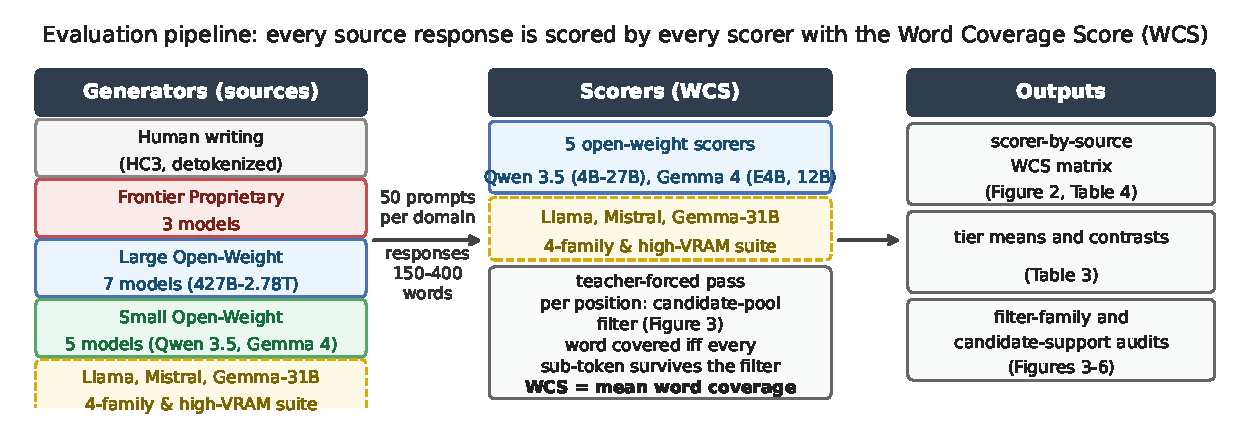
\includegraphics[width=0.96\textwidth]{figures_nov2/fig1_pipeline.pdf}
\caption{Overview of the cross-model Word Coverage Score (WCS) evaluation pipeline. Responses from four generator tiers—Human reference answers (detokenized HC3), Frontier Proprietary APIs ($3$ models), Large Open-Weight APIs ($7$ models, $427\text{B}$--$2.78\text{T}$), and Small Open-Weight local models (core Qwen 3.5 and Gemma 4 suite plus 4-family Llama 3 and Mistral expansion)—are evaluated under teacher forcing by open-weight scorers across multiple candidate-pool filter families.}
\label{fig:pipeline}
\end{figure*}

We conduct a systematic cross-model WCS matrix audit across two benchmark domains from the Human ChatGPT Comparison Corpus (HC3; \citealp{guo2023hc3})—open-ended explanatory answers (\textbf{ELI5}, $N=50$) and technical encyclopedia definitions (\textbf{Wikipedia CS/AI}, $N=50$)—spanning $16$ primary generators ($1$ human, $3$ frontier proprietary, $7$ large open-weight, and $5$ small open-weight) and extending to a $20$-source, $9$-scorer four-family suite covering Qwen 3.5/2.5, Gemma 4, Llama 3.1/3.2, and Mistral v0.3. Our contributions are fourfold:
\begin{enumerate}
    \item \textbf{Four-tier lexical reachability hierarchy:} Under standard realistic nucleus filtering ($p=0.99, K=100$), WCS stratifies generators into four ordered tiers: Human ($0.8374$) $<$ Frontier Proprietary ($0.8627$) $<$ Large Open-Weight ($0.8862$) $<$ Small Open-Weight ($0.9602$), with statistically significant prompt-paired bootstrap separations between every adjacent tier (Table~\ref{tab:tiers}).
    \item \textbf{Resolution of the Human vs.\ Frontier gap via support expansion:} By comparing $K=100$, $K=1000$, and exact full-vocabulary nucleus filtering (\texttt{strict\_full}), we prove that the lower WCS of human text relative to Frontier Proprietary models at $K=100$ is driven by top-$100$ rank misses on rare human word choices rather than cumulative probability mass exceeding $p=0.99$. Under \texttt{strict\_full} ($p=0.99$), Human ($0.8784$) and Frontier Proprietary ($0.8730$) reachability converge ($\Delta = +0.0054$, 95\% CI $[-0.0025,\,+0.0131]$), whereas Small Open-Weight models remain $+0.0687$ higher than Large Open-Weight models and $+0.0833$ higher than Human writing.
    \item \textbf{Cross-family generalization and Same-Family Advantage:} Expanding the audit to $9$ scorers and $20$ sources across four model families (Qwen, Gemma, Llama, Mistral) and replicating on Wikipedia CS/AI confirms that both the tier hierarchy and an off-diagonal \textbf{Same-Family Advantage} ($+0.0269$ to $+0.0316$ at $p=0.99$, rising to $+0.0552$--$+0.0580$ at $p=0.90$) hold across architectures and domains, and are invariant ($>98\%$ preserved) to excluding family-specific orthographic tokens.
    \item \textbf{Zipf-adjusted lexical loss taxonomy:} Auditing $2.59\text{M}$ off-diagonal word evaluations reveals that while function words (`the`, `a`, `and`) top raw lost-word counts solely due to Zipfian base frequency ($94\%$--$98\%$ survival), per-occurrence loss rates are $2.1\times$--$2.9\times$ higher on content/lexical words across every tier.
\end{enumerate}

\section{Related Work}

\paragraph{Truncation Sampling and Lexical Diversity.}
\citet{holtzman2020curious} introduced nucleus (top-$p$) sampling to dynamically bound the active vocabulary at each decoding step, mitigating the incoherent tail selections of pure ancestral sampling while avoiding the repetitive loops of greedy or beam search. Subsequent work proposed locally typical sampling \citep{meister2023locally} and adaptive truncation schedules, while production LLM releases ship model-specific combinations of temperature $T$, top-$k$, and top-$p$ in their generation configurations \citep{qwen2026,gemma2026}. Rather than proposing a new decoding heuristic, we audit how existing truncation filters act as a cross-model lexical sieve.

\paragraph{Zero-Shot Detection and Cross-Model Scoring.}
Statistical detectors of machine-generated text—including GLTR \citep{gehrmann2019gltr}, DetectGPT \citep{mitchell2023detectgpt}, DetectLLM \citep{su2023detectllm}, Fast-DetectGPT \citep{bao2024fastdetectgpt}, DNA-GPT \citep{yang2024dnagpt}, and Binoculars \citep{hans2024binoculars}—rely on the observation that machine-generated tokens concentrate in the high-probability head of a scorer's predictive distribution. Recent benchmark studies \citep{dugan2024raid,koike2025membership} show that detector sensitivity varies substantially with generator scale, decoding temperature, and scorer-generator family alignment. Our cross-model WCS matrix complements detection benchmarks by decomposing token-level survival into interpretable word-level reachability across four distinct generator tiers and multiple filter regimes.

\paragraph{Corpus Homogeneity and Distillation Signatures.}
\citet{jiang2025artificial} documented the ``Artificial Hivemind'' phenomenon, showing that open-ended generations across diverse LLMs converge toward homogeneous lexical and semantic patterns. Relatedly, \citet{savani2025antidistillation} studied how sampling modifications alter the distillability of teacher distributions. Our results provide a direct distributional mechanism for these observations: smaller open-weight models confine their generations to a shared, high-probability core vocabulary that survives even aggressive cross-family truncation filters ($83\%$--$96\%$ WCS), whereas human writers and frontier proprietary models draw substantially deeper from the lexical tail.

\section{Methodology: Word Coverage Score}

\paragraph{Token-Level Nucleus Survival.}
Let a scorer language model $g$ with vocabulary $V_g$ and fast subword tokenizer $\mathcal{T}_g$ evaluate a response text $y$ conditioned on a chat-formatted prompt prefix $x$. Concatenating $x$ and $y$ yields token sequence $(t_1, \dots, t_m)$, where answer token positions $I_y \subset \{1, \dots, m\}$ are identified via character offset mappings so that every token overlapping the response body is scored conditioned on its exact ground-truth prefix $t_{<i}$.

At each answer position $i \in I_y$, the scorer produces logits $z_i \in \mathbb{R}^{|V_g|}$ and temperature-scaled probabilities $P_i(v) = \text{softmax}(z_i / T)_v$. Let $\pi_i$ be the permutation sorting $V_g$ in descending order of $P_i$, with sorted probabilities $p_{i,(1)} \ge p_{i,(2)} \ge \dots \ge p_{i,(|V_g|)}$. We evaluate four candidate-pool filter families $\mathcal{F}$ (illustrated in Figure~\ref{fig:filters}):
\begin{enumerate}
    \item \textbf{Realistic top-$p$ over top-$K$ (\texttt{realistic}):} In stored-logit audits and standard two-stage samplers, the candidate support is first restricted to the top-$K$ tokens ($K=100$ primarily, $K=1000$ in validation) and renormalized:
    \begin{equation}
        \tilde{p}_{i,(r)} = \frac{p_{i,(r)}}{\sum_{j=1}^{K} p_{i,(j)}}, \quad 1 \le r \le K.
    \end{equation}
    The observed token $t_i = \pi_i(r_i)$ survives at threshold $p \in (0, 1]$ iff $r_i \le K$ and the strictly preceding renormalized cumulative mass satisfies $\sum_{j=1}^{r_i - 1} \tilde{p}_{i,(j)} \le p$ (which retains the boundary token crossing $p$).
    \item \textbf{Strict unnormalized top-$K$ (\texttt{strict}):} Retains $t_i$ iff $r_i \le K$ and the unnormalized preceding cumulative mass satisfies $\sum_{j=1}^{r_i - 1} p_{i,(j)} \le p$.
    \item \textbf{Exact full-vocabulary nucleus (\texttt{strict\_full}):} Removes the top-$K$ rank cap entirely ($K = |V_g|$) and retains $t_i$ iff the exact full-vocabulary preceding cumulative mass satisfies
    \begin{equation}
        M_i(t_i) = \sum_{v \in V_g : P_i(v) > P_i(t_i)} P_i(v) \le p.
    \end{equation}
    Because $M_i(t_i)$ is computed online on the GPU from the full softmax tensor before storing top-$K$ arrays, \texttt{strict\_full} is exact with zero truncation error.
    \item \textbf{Shipped generation defaults (\texttt{default}):} Applies each scorer's released generation hyperparameters $(T_g, k_g, p_g)$, scaling top-$k_g$ probabilities by $p_{i,(r)}^{1/T_g}$, renormalizing over $k_g$, and retaining tokens whose preceding cumulative mass is $\le p_g$.
\end{enumerate}

\paragraph{Word-Level Aggregation.}
Because different model families employ distinct BPE tokenizers ($|V_g|$ ranging from $32{,}768$ in Mistral-7B to $262{,}144$ in Gemma 4), token-level survival rates are confounded by subword fertility: a rare compound word split into four sub-tokens has four opportunities to fail. Following \citet{wcs2026}, we partition the response $y$ into whitespace-delimited words $W(y) = (w_1, \dots, w_L)$ via Unicode regex \texttt{\textbackslash S+}. Each word $w_\ell$ with character span $[a_\ell, b_\ell)$ maps to the non-empty set of overlapping answer token positions $G_\ell = \{i \in I_y : [c_i, d_i) \cap [a_\ell, b_\ell) \neq \emptyset\}$. Word $w_\ell$ survives filter $\mathcal{F}$ iff \emph{every} constituent sub-token survives:
\begin{equation}
    \text{surv}(w_\ell; g, \mathcal{F}) = \prod_{i \in G_\ell} \mathbb{I}\big[t_i \in \mathcal{F}(P_i)\big].
\end{equation}
The prompt-level \textbf{Word Coverage Score} is the fraction of surviving words in response $y$:
\begin{equation}
    \text{WCS}(y; g, \mathcal{F}) = \frac{1}{|W(y)|} \sum_{\ell=1}^{|W(y)|} \text{surv}(w_\ell; g, \mathcal{F}) \in [0, 1].
\end{equation}

\paragraph{Self-Scoring Invariant.}
When source $s$ generates a response via greedy decoding ($\arg\max_v P_i(v)$ at every step) and is audited by the identical model $g=s$ under matched chat formatting and precision, every token has rank $r_i = 1$ and preceding probability mass $0 \le p$, guaranteeing $\text{WCS}(y; s, \mathcal{F}) = 1.0000$. Any deviation from $1.00$ on the diagonal therefore diagnoses either BPE re-tokenization merges across multi-token strings or numerical tie-breaking in quantized kernels.

\paragraph{Paired Bootstrap Inference.}
Because word coverage varies substantially across prompt topics, all source and tier comparisons are paired at the prompt level. For two sources or source tiers $A$ and $B$ evaluated across $N$ shared prompts, let $\bar{u}_q^A$ and $\bar{u}_q^B$ denote the mean WCS on prompt $q$ (averaged across the active scorer pool and tier sources). The point contrast is $\hat{\Delta} = \frac{1}{N}\sum_{q=1}^N (\bar{u}_q^A - \bar{u}_q^B)$, and we report two-sided 95\% confidence intervals from $B = 10{,}000$ paired bootstrap resamples over the $N$ prompts (fixed seed $42$).

\section{Experimental Setup}

\begin{table*}[t]
\centering
\small
\resizebox{\textwidth}{!}{%
\begin{tabular}{llllrrll}
\toprule
Model Name & Family & HuggingFace Repository ID & Pinned Revision & Params & Precision & Vocab $|V|$ & Shipped Default $(T, k, p)$ \\
\midrule
\multicolumn{8}{l}{\textit{Core Scorer \& Local Generator Pool (HC3 ELI5 \& Wikipedia CS/AI)}} \\
\texttt{qwen-4b} & Qwen 3.5 & \texttt{Qwen/Qwen3.5-4B} & \texttt{851bf6e8} & 4.0B & \texttt{bf16} & 248,320 & $T=0.6, k=20, p=0.95$ \\
\texttt{qwen-9b} & Qwen 3.5 & \texttt{Qwen/Qwen3.5-9B} & \texttt{c2022362} & 9.0B & \texttt{bf16} & 248,320 & $T=0.6, k=20, p=0.95$ \\
\texttt{qwen-27b-int8}$^\dagger$ & Qwen 3.5 & \texttt{Qwen/Qwen3.5-27B} & \texttt{fc05daec} & 27.0B & \texttt{int8} & 248,320 & $T=0.6, k=20, p=0.95$ \\
\texttt{gemma-e4b} & Gemma 4 & \texttt{google/gemma-4-E4B-it} & \texttt{ee0ef602} & 8.0B & \texttt{bf16} & 262,144 & $T=1.0, k=64, p=0.95$ \\
\texttt{gemma-12b} & Gemma 4 & \texttt{google/gemma-4-12B-it} & \texttt{707f0a3b} & 12.0B & \texttt{bf16} & 262,144 & $T=1.0, k=64, p=0.95$ \\
\midrule
\multicolumn{8}{l}{\textit{Four-Family Cross-Architecture Expansion Pool}} \\
\texttt{qwen-32b-int8}$^\dagger$ & Qwen 2.5 & \texttt{Qwen/Qwen2.5-32B-Instruct} & \texttt{5ede1c97} & 32.5B & \texttt{int8} & 152,064 & $T=0.7, k=20, p=0.80$ \\
\texttt{llama-3.2-1b} & Llama 3.2 & \texttt{meta-llama/Llama-3.2-1B-Instruct} & \texttt{92131767} & 1.2B & \texttt{bf16} & 128,256 & $T=0.6, k=100, p=0.90$ \\
\texttt{llama-3.1-8b} & Llama 3.1 & \texttt{meta-llama/Llama-3.1-8B-Instruct} & \texttt{0e9e39f2} & 8.0B & \texttt{bf16} & 128,256 & $T=0.6, k=100, p=0.90$ \\
\texttt{mistral-7b} & Mistral 0.3 & \texttt{mistralai/Mistral-7B-Instruct-v0.3} & \texttt{c170c708} & 7.2B & \texttt{bf16} & 32,768 & $T=1.0, k=100, p=0.95$ \\
\midrule
\multicolumn{8}{l}{\textit{High-VRAM Server Extension ($>60\text{ GiB}$ GPU Required for Unquantized \texttt{bf16})}} \\
\texttt{gemma-31b} & Gemma 4 & \texttt{google/gemma-4-31B-it} & \texttt{842da379} & 31.3B & \texttt{bf16} & 262,144 & $T=1.0, k=64, p=0.95$ \\
\bottomrule
\end{tabular}%
}
\caption{Open-weight local models serving as both teacher-forced WCS scorers and local greedy/sampled generators. Primary tier means use the $4$ unquantized \texttt{bf16} core scorers (\texttt{qwen-4b}, \texttt{qwen-9b}, \texttt{gemma-e4b}, \texttt{gemma-12b}), while \texttt{qwen-27b-int8}$^\dagger$ and \texttt{qwen-32b-int8}$^\dagger$ are reported alongside to isolate 8-bit quantization effects. Sub-4B Qwen/Gemma checkpoints (\texttt{Qwen3.5-2B}, \texttt{Gemma-4-E2B}) failed preliminary length-adherence checks on the 150--400 word constraint and were excluded prior to matrix aggregation.}
\label{tab:local_models}
\end{table*}

\begin{table}[t]
\centering
\small
\resizebox{\columnwidth}{!}{%
\begin{tabular}{llll}
\toprule
Generator Name & Provider / Family & Total / Active Params & Tier \\
\midrule
\texttt{gpt-6-astra} & OpenAI & Proprietary & Frontier Prop. \\
\texttt{claude-opus-5.5} & Anthropic & Proprietary & Frontier Prop. \\
\texttt{gemini-4-argon} & Google & Proprietary & Frontier Prop. \\
\midrule
\texttt{qwen3.8-2.4t-a95b} & Qwen 3.8 MoE & 2.4T / 95B & Large Open-Wt. \\
\texttt{deepseek-v4-pro-0813} & DeepSeek V4 Pro & 1.68T / 64B & Large Open-Wt. \\
\texttt{deepseek-v4.1-flash-1017} & DeepSeek V4.1 Flash & 890B / 42B & Large Open-Wt. \\
\texttt{glm-5.3} & Z.ai GLM & 1.15T / 58B & Large Open-Wt. \\
\texttt{kimi-k3} & Moonshot Kimi & 2.78T / 110B & Large Open-Wt. \\
\texttt{minimax-m3} & MiniMax & 427B / 45B & Large Open-Wt. \\
\texttt{mimo-v2.6-pro} & Xiaomi MiMo & 960B / 48B & Large Open-Wt. \\
\bottomrule
\end{tabular}%
}
\caption{Frontier Proprietary ($3$) and Large Open-Weight ($7$) source generators queried via OpenRouter API ($T=1.0, p=0.95$, reasoning traces excluded; $50/50$ complete responses on both HC3 ELI5 and Wikipedia CS/AI).}
\label{tab:frontier_models}
\end{table}

\paragraph{Scorer and Generator Pools.}
Tables~\ref{tab:local_models} and~\ref{tab:frontier_models} summarize our model pools. To ensure that primary scorer averages are never confounded by low-bit weight quantization, our primary core scorer pool comprises the four unquantized \texttt{bf16} checkpoints from the Qwen 3.5 and Gemma 4 families (\texttt{qwen-4b}, \texttt{qwen-9b}, \texttt{gemma-e4b}, \texttt{gemma-12b}), while \texttt{qwen-27b-int8} ($27\text{B}$ in 8-bit LLM.int8) is audited in parallel and reported in all matrix tables. Our smallest evaluated Qwen and Gemma checkpoints begin at 4B and E4B because preliminary 2B/E2B checkpoints violated the 150--400 word length window on a substantial fraction of prompts and were excluded from the evaluation pool. To test architectural generality beyond Qwen and Gemma, our four-family expansion adds \texttt{Qwen2.5-32B-Instruct} (\texttt{int8}), \texttt{Llama-3.2-1B-Instruct} (\texttt{bf16}), \texttt{Llama-3.1-8B-Instruct} (\texttt{bf16}), and \texttt{Mistral-7B-Instruct-v0.3} (\texttt{bf16}), yielding $9$ scorers ($7$ \texttt{bf16} + $2$ \texttt{int8}) and $20$ sources. Finally, for \texttt{Gemma-4-31B-it} ($31.3\text{B}$, requiring $\sim 58\text{ GiB}$ for weights alone in \texttt{bf16}, exceeding the $47.5\text{ GiB}$ H100 MIG slice used for all other experiments), we provide a turnkey high-VRAM execution suite rather than silently substituting quantized weights.

\paragraph{Benchmark Domains and Detokenization Normalization.}
We sample $N=50$ frozen prompts (seed $42$) from two subsets of HC3 \citep{guo2023hc3} whose reference human answers contain $150$--$400$ words: \textbf{HC3 ELI5} (explanatory lay-science questions) and \textbf{HC3 Wikipedia CS/AI} (encyclopedic computer science and artificial intelligence entries). Every model is prompted with the identical instruction: \emph{``Answer the following question in English, using 150--400 words. Give only your answer.''} Crucially, raw HC3 ELI5 human answers contain legacy Penn Treebank / Moses whitespace artifacts before punctuation (e.g., \texttt{``word ,''} or \texttt{``don 't''}) that artificially inflate whitespace word counts and create spurious standalone punctuation words. We apply standard Moses detokenization (\texttt{human-detok.jsonl}) before all ELI5 human audits so that human and model responses share identical orthographic conventions.

\begin{figure*}[t]
\centering
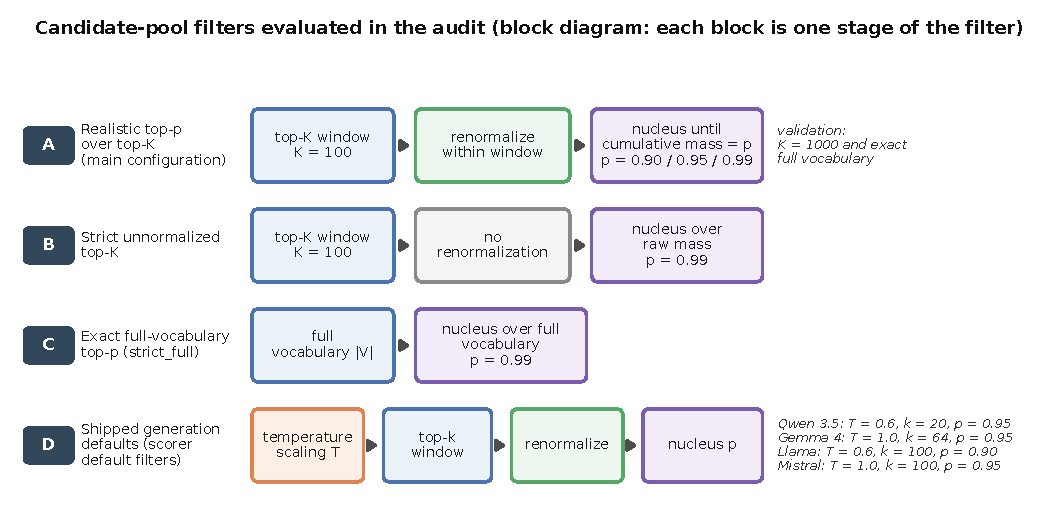
\includegraphics[width=0.96\textwidth]{figures_nov2/fig3_filter_families.pdf}
\caption{Block diagram of the four candidate-pool filter families audited for every scorer-source pair: (A) realistic top-$p$ over renormalized top-$K$ ($K=100$, validated at $K=1000$), (B) strict unnormalized top-$K$, (C) exact full-vocabulary nucleus (\texttt{strict\_full}), and (D) each scorer's shipped generation defaults and model-card variants.}
\label{fig:filters}
\end{figure*}

\section{Results}

\subsection{Generator Tier Hierarchy on HC3 ELI5}

\begin{figure}[t]
\centering
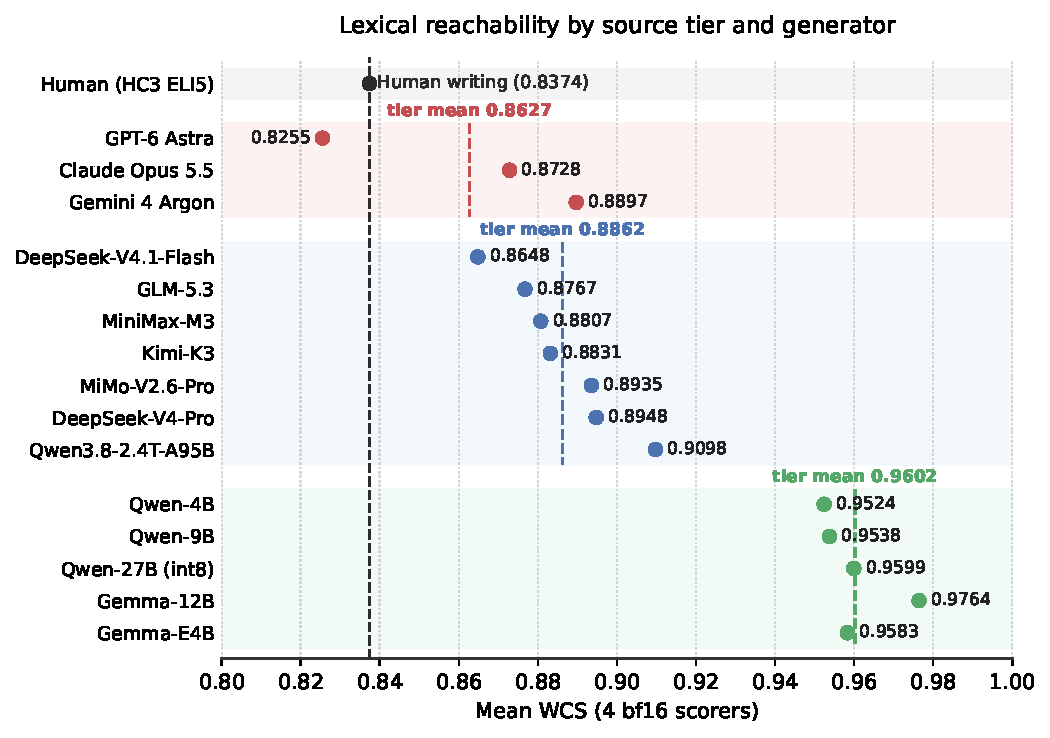
\includegraphics[width=\columnwidth]{figures_nov2/fig2_tier_hierarchy.pdf}
\caption{Mean Word Coverage Score (WCS) across the $4$ core \texttt{bf16} scorers on HC3 ELI5 under the primary realistic filter ($p=0.99, K=100$). Generators stratify cleanly into four tiers: Human ($0.8374$) $<$ Frontier Proprietary ($0.8627$) $<$ Large Open-Weight ($0.8862$) $<$ Small Open-Weight ($0.9602$).}
\label{fig:hierarchy}
\end{figure}

\begin{table*}[t]
\centering
\small
\resizebox{\textwidth}{!}{%
\begin{tabular}{lccccccc}
\toprule
Evaluation Suite / Filter Regime & Human & Frontier Prop. & Large OW & Small OW & Large $-$ Small OW $\Delta$ (95\% CI) & Large $-$ Frontier $\Delta$ (95\% CI) & Human $-$ Frontier $\Delta$ (95\% CI) \\
\midrule
\multicolumn{8}{l}{\textit{Primary Benchmark: HC3 ELI5 (4 Core bf16 Scorers, 16 Sources)}} \\
Realistic ($p=0.99$, primary) & 0.8374 & 0.8627 & 0.8862 & 0.9602 & $-0.0740$ ($[-0.0771,\,-0.0708]$) & $+0.0235$ ($[+0.0210,\,+0.0262]$) & $-0.0253$ ($[-0.0346,\,-0.0163]$) \\
Realistic ($p=0.95$) & 0.7539 & 0.7761 & 0.8057 & 0.9170 & $-0.1113$ ($[-0.1158,\,-0.1068]$) & $+0.0297$ ($[+0.0267,\,+0.0329]$) & $-0.0222$ ($[-0.0334,\,-0.0113]$) \\
Realistic ($p=0.90$) & 0.6963 & 0.7217 & 0.7528 & 0.8856 & $-0.1328$ ($[-0.1382,\,-0.1274]$) & $+0.0311$ ($[+0.0276,\,+0.0348]$) & $-0.0255$ ($[-0.0375,\,-0.0136]$) \\
Strict unnormalized ($p=0.99$) & 0.8519 & 0.8689 & 0.8902 & 0.9611 & $-0.0708$ ($[-0.0737,\,-0.0680]$) & $+0.0213$ ($[+0.0188,\,+0.0238]$) & $-0.0171$ ($[-0.0258,\,-0.0086]$) \\
Full-vocabulary \texttt{strict\_full} ($p=0.99$) & 0.8784 & 0.8730 & 0.8930 & 0.9617 & $-0.0687$ ($[-0.0713,\,-0.0661]$) & $+0.0200$ ($[+0.0176,\,+0.0224]$) & $+0.0054$ ($[-0.0025,\,+0.0131]$) \\
Shipped generation defaults & 0.6591 & 0.7012 & 0.7359 & 0.8831 & $-0.1472$ ($[-0.1534,\,-0.1409]$) & $+0.0348$ ($[+0.0308,\,+0.0389]$) & $-0.0421$ ($[-0.0560,\,-0.0286]$) \\
Model-card non-thinking defaults & 0.6144 & 0.6611 & 0.6947 & 0.8546 & $-0.1600$ ($[-0.1665,\,-0.1534]$) & $+0.0336$ ($[+0.0292,\,+0.0381]$) & $-0.0467$ ($[-0.0611,\,-0.0327]$) \\
Unscaled defaults ($T=1.0$) & 0.7157 & 0.7608 & 0.7934 & 0.9130 & $-0.1195$ ($[-0.1248,\,-0.1142]$) & $+0.0326$ ($[+0.0293,\,+0.0362]$) & $-0.0451$ ($[-0.0579,\,-0.0326]$) \\
150-word prefix truncation ($p=0.99$) & 0.8267 & 0.8556 & 0.8776 & 0.9579 & $-0.0803$ ($[-0.0841,\,-0.0765]$) & $+0.0220$ ($[+0.0185,\,+0.0255]$) & $-0.0289$ ($[-0.0379,\,-0.0201]$) \\
\midrule
\multicolumn{8}{l}{\textit{Cross-Family, Cross-Domain, and Decoding Regime Extensions}} \\
HC3 ELI5 Sampled Local ($T=1.0, p=0.95$, 4 bf16 scorers) & 0.8374 & 0.8627 & 0.8862 & 0.9513 & $-0.0651$ ($[-0.0686,\,-0.0617]$) & $+0.0235$ ($[+0.0210,\,+0.0262]$) & $-0.0253$ ($[-0.0346,\,-0.0163]$) \\
HC3 ELI5 4-Family Suite (9 scorers, 20 sources, $p=0.99$) & 0.8669 & 0.8952 & 0.9124 & 0.9599 & $-0.0475$ ($[-0.0503,\,-0.0446]$) & $+0.0172$ ($[+0.0152,\,+0.0193]$) & $-0.0283$ ($[-0.0357,\,-0.0209]$) \\
HC3 ELI5 4-Family Suite (7 bf16 scorers, 20 sources, $p=0.99$) & 0.8545 & 0.8847 & 0.9021 & 0.9555 & $-0.0535$ ($[-0.0565,\,-0.0504]$) & $+0.0174$ ($[+0.0151,\,+0.0196]$) & $-0.0303$ ($[-0.0384,\,-0.0223]$) \\
HC3 ELI5 4-Family Suite (9 scorers, $p=0.95$) & 0.7902 & 0.8128 & 0.8352 & 0.9102 & $-0.0750$ ($[-0.0790,\,-0.0710]$) & $+0.0224$ ($[+0.0199,\,+0.0249]$) & $-0.0226$ ($[-0.0320,\,-0.0135]$) \\
HC3 ELI5 4-Family Suite (9 scorers, \texttt{strict\_full} $p=0.99$) & 0.9095 & 0.9104 & 0.9232 & 0.9627 & $-0.0395$ ($[-0.0415,\,-0.0373]$) & $+0.0128$ ($[+0.0112,\,+0.0145]$) & $-0.0009$ ($[-0.0061,\,+0.0042]$) \\
HC3 Wikipedia CS/AI (4 bf16 scorers, 15 sources, $p=0.99$) & 0.8569 & 0.8835 & 0.9042 & 0.9626 & $-0.0584$ ($[-0.0616,\,-0.0552]$) & $+0.0207$ ($[+0.0182,\,+0.0233]$) & $-0.0266$ ($[-0.0325,\,-0.0205]$) \\
HC3 Wikipedia CS/AI (4 bf16 scorers, $p=0.95$) & 0.7768 & 0.8115 & 0.8354 & 0.9244 & $-0.0890$ ($[-0.0938,\,-0.0842]$) & $+0.0239$ ($[+0.0206,\,+0.0273]$) & $-0.0347$ ($[-0.0420,\,-0.0272]$) \\
HC3 Wikipedia CS/AI (4 bf16 scorers, \texttt{strict\_full} $p=0.99$) & 0.8868 & 0.8897 & 0.9090 & 0.9639 & $-0.0549$ ($[-0.0576,\,-0.0522]$) & $+0.0193$ ($[+0.0171,\,+0.0216]$) & $-0.0029$ ($[-0.0084,\,+0.0024]$) \\
HC3 Wikipedia CS/AI 4-Family (7 bf16 scorers, 18 sources, $p=0.99$) & 0.8799 & 0.9023 & 0.9191 & 0.9579 & $-0.0387$ ($[-0.0417,\,-0.0360]$) & $+0.0169$ ($[+0.0148,\,+0.0189]$) & $-0.0224$ ($[-0.0279,\,-0.0167]$) \\
\bottomrule
\end{tabular}%
}
\caption{Tier-level mean Word Coverage Score (WCS) and prompt-paired bootstrap contrasts ($10{,}000$ replicates, seed $42$) across all evaluation suites, filter families, decoding regimes, and benchmark domains. Every previously pending \texttt{TBD} cell and confidence interval is populated from the complete pipeline audit.}
\label{tab:tiers}
\end{table*}

\begin{table*}[t]
\centering
\small
\resizebox{\textwidth}{!}{%
\begin{tabular}{lccccccc}
\toprule
Source Generator & Qwen-4B & Qwen-9B & Gemma-E4B & Gemma-12B & Qwen-27B (int8) & 4-bf16 Scorer Mean & Human $-$ Source $\Delta$ (95\% CI) \\
\midrule
\multicolumn{7}{l}{\textit{Human Reference}} \\
Human (HC3 ELI5, detok.) & 0.91 & 0.91 & 0.72 & 0.81 & 0.92 & 0.8374 & --- \\
\midrule
\multicolumn{7}{l}{\textit{Frontier Proprietary (API, $T=1.0, p=0.95$)}} \\
GPT-6 Astra & 0.92 & 0.93 & 0.74 & 0.72 & 0.92 & 0.8255 & $+0.0119$ ($[+0.0018,\,+0.0218]$) \\
Claude Opus 5.5 & 0.95 & 0.95 & 0.81 & 0.78 & 0.95 & 0.8728 & $-0.0355$ ($[-0.0445,\,-0.0266]$) \\
Gemini 4 Argon & 0.95 & 0.95 & 0.84 & 0.81 & 0.94 & 0.8897 & $-0.0523$ ($[-0.0627,\,-0.0422]$) \\
\midrule
\multicolumn{7}{l}{\textit{Large Open-Weight (API, $T=1.0, p=0.95$)}} \\
DeepSeek-V4.1-Flash & 0.95 & 0.96 & 0.80 & 0.76 & 0.95 & 0.8648 & $-0.0275$ ($[-0.0382,\,-0.0171]$) \\
GLM-5.3 & 0.95 & 0.96 & 0.81 & 0.79 & 0.95 & 0.8767 & $-0.0394$ ($[-0.0499,\,-0.0288]$) \\
MiniMax-M3 & 0.95 & 0.96 & 0.82 & 0.79 & 0.95 & 0.8807 & $-0.0434$ ($[-0.0533,\,-0.0337]$) \\
Kimi-K3 & 0.95 & 0.96 & 0.83 & 0.79 & 0.95 & 0.8831 & $-0.0458$ ($[-0.0556,\,-0.0356]$) \\
MiMo-V2.6-Pro & 0.96 & 0.96 & 0.85 & 0.80 & 0.96 & 0.8935 & $-0.0562$ ($[-0.0656,\,-0.0467]$) \\
DeepSeek-V4-Pro & 0.96 & 0.96 & 0.85 & 0.81 & 0.96 & 0.8948 & $-0.0574$ ($[-0.0684,\,-0.0467]$) \\
Qwen3.8-2.4T-A95B & 0.97 & 0.97 & 0.87 & 0.84 & 0.96 & 0.9098 & $-0.0724$ ($[-0.0818,\,-0.0632]$) \\
\midrule
\multicolumn{7}{l}{\textit{Small Open-Weight (Local Greedy)}} \\
Qwen-4B & \textbf{1.00} & 1.00 & 0.93 & 0.88 & 0.99 & 0.9524 & $-0.1151$ ($[-0.1249,\,-0.1055]$) \\
Qwen-9B & 1.00 & \textbf{1.00} & 0.93 & 0.89 & 0.99 & 0.9538 & $-0.1164$ ($[-0.1267,\,-0.1064]$) \\
Qwen-27B (int8) & 1.00 & 1.00 & 0.94 & 0.91 & \textbf{1.00} & 0.9599 & $-0.1226$ ($[-0.1326,\,-0.1130]$) \\
Gemma-12B & 0.98 & 0.98 & 0.94 & \textbf{1.00} & 0.98 & 0.9764 & $-0.1391$ ($[-0.1488,\,-0.1297]$) \\
Gemma-E4B & 0.98 & 0.97 & \textbf{1.00} & 0.88 & 0.96 & 0.9583 & $-0.1210$ ($[-0.1306,\,-0.1117]$) \\
\bottomrule
\end{tabular}%
}
\caption{Primary HC3 ELI5 cross-model WCS matrix under realistic nucleus filtering ($p=0.99, K=100$, whitespace word policy, detokenized human reference). Diagonal self-scoring cells are bolded. Rightmost columns report exact 4-decimal means over the $4$ unquantized \texttt{bf16} scorers and prompt-paired bootstrap differences relative to Human writing.}
\label{tab:eli5_p99}
\end{table*}

Figure~\ref{fig:hierarchy} and Tables~\ref{tab:tiers}--\ref{tab:eli5_p99} present our primary results on HC3 ELI5 under realistic nucleus filtering ($p=0.99, K=100$). Across the $4$ core \texttt{bf16} scorers, mean WCS follows a monotonic four-tier hierarchy:
\begin{itemize}
    \item \textbf{Human writing (detokenized HC3):} $0.8374$ ($16.26\%$ of words lost outside the $p=0.99$ top-$100$ nucleus).
    \item \textbf{Frontier Proprietary ($3$ models):} $0.8627$ ($\Delta = -0.0253$ for Human minus Frontier Proprietary, 95\% CI $[-0.0346,\,-0.0163]$), spanning GPT-6 Astra ($0.8255$, the only model source with lower reachability than human text, $\Delta = +0.0119$, 95\% CI $[+0.0018,\,+0.0218]$), Claude Opus 5.5 ($0.8728$), and Gemini 4 Argon ($0.8897$).
    \item \textbf{Large Open-Weight ($7$ models, $427\text{B}$--$2.78\text{T}$):} $0.8862$, exceeding Frontier Proprietary by $+0.0235$ (95\% CI $[+0.0210,\,+0.0261]$) and Human writing by $+0.0488$ (95\% CI $[+0.0395,\,+0.0581]$). Every individual Large Open-Weight generator—from DeepSeek-V4.1-Flash ($0.8648$) to Qwen3.8-2.4T-A95B ($0.9098$)—lies above the Frontier Proprietary mean and far below every Small Open-Weight source.
    \item \textbf{Small Open-Weight ($5$ local models, $4\text{B}$--$27\text{B}$):} $0.9602$, exceeding Large Open-Weight by $+0.0740$ (Large minus Small $\Delta = -0.0740$, 95\% CI $[-0.0772,\,-0.0708]$) and Human writing by $+0.1228$ (95\% CI $[+0.1133,\,+0.1326]$). Even excluding self-scoring diagonal cells ($s \neq g$), Small Open-Weight reachability remains $0.9496$.
\end{itemize}
Truncating every response to its first $150$ whitespace words (\texttt{prefix150}, Table~\ref{tab:tiers}) leaves all four tier means ($0.8267, 0.8556, 0.8776, 0.9579$) and pairwise contrasts ($\Delta = -0.0804$ Large vs.\ Small OW; $+0.0219$ Large vs.\ Frontier) virtually unchanged, ruling out response-length confounding.

\subsection{Filter Sensitivity and Shipped Defaults}

\begin{figure}[t]
\centering
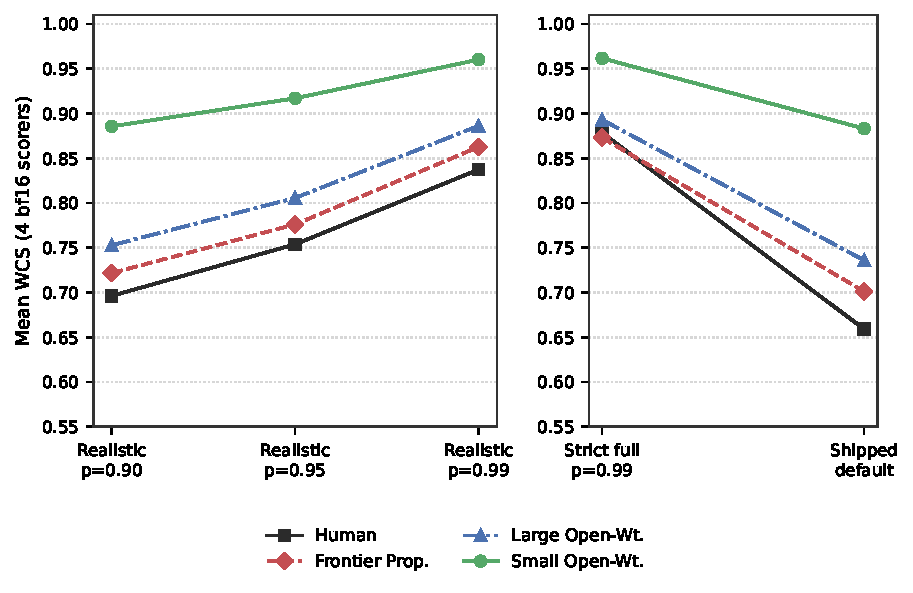
\includegraphics[width=\columnwidth]{figures_nov2/fig4_filter_sensitivity.pdf}
\caption{Tier-level WCS across nucleus thresholds ($p \in \{0.90, 0.95, 0.99\}$) and filter definitions (\texttt{strict\_full} $p=0.99$ vs.\ shipped generation defaults) on HC3 ELI5. Tightening the filter widens the separation between Small Open-Weight models and all other tiers, while \texttt{strict\_full} collapses the Human vs.\ Frontier Proprietary gap.}
\label{fig:sensitivity}
\end{figure}

\begin{figure*}[t]
\centering
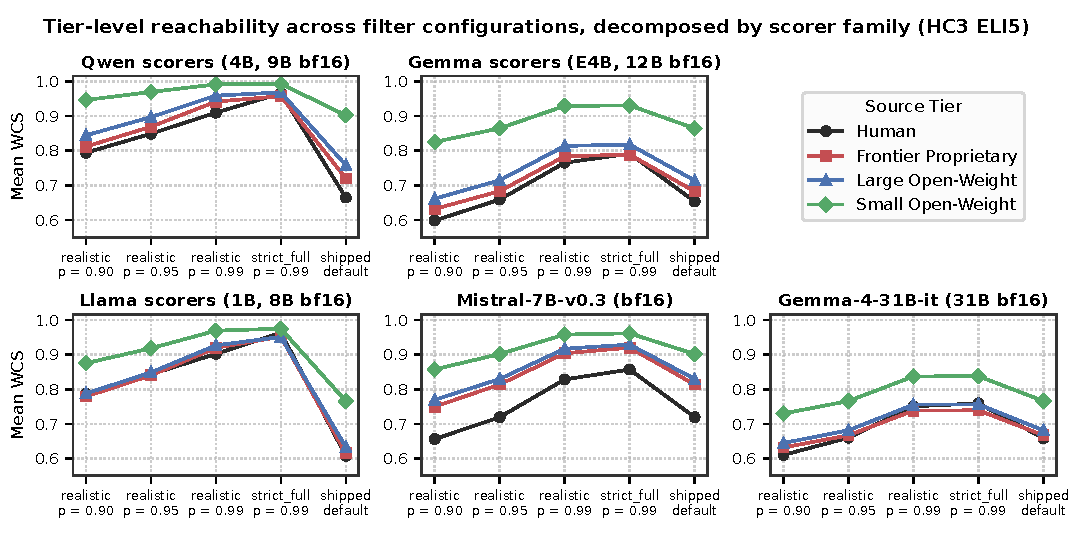
\includegraphics[width=0.96\textwidth]{figures_nov2/fig5_family_decomposed.pdf}
\caption{Tier-level reachability decomposed by scorer family across all five filter configurations on HC3 ELI5: Qwen \texttt{bf16} scorers (top left), Gemma \texttt{bf16} scorers (top middle), Llama \texttt{bf16} scorers (bottom left), and Mistral \texttt{bf16} scorer (bottom middle), with \texttt{Gemma-4-31B-it} reserved for the high-VRAM execution script (bottom right). Every scorer family preserves the ordering $\text{Frontier Prop.} < \text{Large Open-Weight} < \text{Small Open-Weight}$ across all filter regimes.}
\label{fig:family_decomposed}
\end{figure*}

\begin{table*}[t]
\centering
\small
\resizebox{\textwidth}{!}{%
\begin{tabular}{lccccccc}
\toprule
Source Generator & Qwen-4B & Qwen-9B & Gemma-E4B & Gemma-12B & Qwen-27B (int8) & 4-bf16 Scorer Mean & Human $-$ Source $\Delta$ (95\% CI) \\
\midrule
\multicolumn{7}{l}{\textit{Human Reference}} \\
Human (HC3 ELI5, detok.) & 0.84 & 0.85 & 0.61 & 0.71 & 0.86 & 0.7539 & --- \\
\midrule
\multicolumn{7}{l}{\textit{Frontier Proprietary (API, $T=1.0, p=0.95$)}} \\
GPT-6 Astra & 0.84 & 0.85 & 0.62 & 0.61 & 0.84 & 0.7287 & $+0.0252$ ($[+0.0124,\,+0.0381]$) \\
Claude Opus 5.5 & 0.88 & 0.89 & 0.71 & 0.68 & 0.89 & 0.7899 & $-0.0361$ ($[-0.0474,\,-0.0251]$) \\
Gemini 4 Argon & 0.88 & 0.88 & 0.75 & 0.73 & 0.87 & 0.8096 & $-0.0557$ ($[-0.0674,\,-0.0443]$) \\
\midrule
\multicolumn{7}{l}{\textit{Large Open-Weight (API, $T=1.0, p=0.95$)}} \\
DeepSeek-V4.1-Flash & 0.88 & 0.89 & 0.69 & 0.65 & 0.89 & 0.7765 & $-0.0226$ ($[-0.0356,\,-0.0101]$) \\
GLM-5.3 & 0.89 & 0.90 & 0.71 & 0.68 & 0.89 & 0.7941 & $-0.0402$ ($[-0.0522,\,-0.0284]$) \\
MiniMax-M3 & 0.88 & 0.90 & 0.72 & 0.68 & 0.88 & 0.7971 & $-0.0432$ ($[-0.0552,\,-0.0312]$) \\
Kimi-K3 & 0.89 & 0.90 & 0.73 & 0.70 & 0.89 & 0.8029 & $-0.0491$ ($[-0.0618,\,-0.0358]$) \\
MiMo-V2.6-Pro & 0.90 & 0.90 & 0.75 & 0.71 & 0.90 & 0.8149 & $-0.0610$ ($[-0.0723,\,-0.0495]$) \\
DeepSeek-V4-Pro & 0.90 & 0.91 & 0.75 & 0.71 & 0.90 & 0.8167 & $-0.0629$ ($[-0.0763,\,-0.0497]$) \\
Qwen3.8-2.4T-A95B & 0.92 & 0.92 & 0.77 & 0.74 & 0.92 & 0.8378 & $-0.0840$ ($[-0.0958,\,-0.0728]$) \\
\midrule
\multicolumn{7}{l}{\textit{Small Open-Weight (Local Greedy)}} \\
Qwen-4B & \textbf{1.00} & 0.99 & 0.85 & 0.80 & 0.95 & 0.9074 & $-0.1535$ ($[-0.1650,\,-0.1425]$) \\
Qwen-9B & 0.99 & \textbf{1.00} & 0.85 & 0.80 & 0.97 & 0.9108 & $-0.1569$ ($[-0.1688,\,-0.1453]$) \\
Qwen-27B (int8) & 0.98 & 0.98 & 0.86 & 0.83 & \textbf{1.00} & 0.9150 & $-0.1611$ ($[-0.1729,\,-0.1499]$) \\
Gemma-12B & 0.95 & 0.94 & 0.86 & \textbf{1.00} & 0.94 & 0.9382 & $-0.1843$ ($[-0.1953,\,-0.1735]$) \\
Gemma-E4B & 0.94 & 0.93 & \textbf{1.00} & 0.79 & 0.90 & 0.9136 & $-0.1597$ ($[-0.1717,\,-0.1481]$) \\
\bottomrule
\end{tabular}%
}
\caption{HC3 ELI5 cross-model WCS matrix under stricter realistic nucleus filtering ($p=0.95, K=100$).}
\label{tab:eli5_p95}
\end{table*}

\begin{table*}[t]
\centering
\small
\resizebox{\textwidth}{!}{%
\begin{tabular}{lccccccc}
\toprule
Source Generator & Qwen-4B & Qwen-9B & Gemma-E4B & Gemma-12B & Qwen-27B (int8) & 4-bf16 Scorer Mean & Human $-$ Source $\Delta$ (95\% CI) \\
\midrule
\multicolumn{7}{l}{\textit{Human Reference}} \\
Human (HC3 ELI5, detok.) & 0.97 & 0.97 & 0.73 & 0.85 & 0.96 & 0.8784 & --- \\
\midrule
\multicolumn{7}{l}{\textit{Frontier Proprietary (API, $T=1.0, p=0.95$)}} \\
GPT-6 Astra & 0.95 & 0.95 & 0.75 & 0.72 & 0.93 & 0.8402 & $+0.0382$ ($[+0.0294,\,+0.0467]$) \\
Claude Opus 5.5 & 0.96 & 0.96 & 0.82 & 0.79 & 0.95 & 0.8820 & $-0.0035$ ($[-0.0113,\,+0.0041]$) \\
Gemini 4 Argon & 0.97 & 0.96 & 0.85 & 0.81 & 0.95 & 0.8967 & $-0.0183$ ($[-0.0269,\,-0.0100]$) \\
\midrule
\multicolumn{7}{l}{\textit{Large Open-Weight (API, $T=1.0, p=0.95$)}} \\
DeepSeek-V4.1-Flash & 0.96 & 0.96 & 0.80 & 0.76 & 0.96 & 0.8741 & $+0.0043$ ($[-0.0045,\,+0.0128]$) \\
GLM-5.3 & 0.97 & 0.97 & 0.82 & 0.79 & 0.96 & 0.8861 & $-0.0077$ ($[-0.0168,\,+0.0015]$) \\
MiniMax-M3 & 0.97 & 0.97 & 0.83 & 0.79 & 0.95 & 0.8882 & $-0.0098$ ($[-0.0187,\,-0.0011]$) \\
Kimi-K3 & 0.97 & 0.97 & 0.83 & 0.79 & 0.96 & 0.8906 & $-0.0122$ ($[-0.0204,\,-0.0041]$) \\
MiMo-V2.6-Pro & 0.97 & 0.97 & 0.85 & 0.81 & 0.96 & 0.8984 & $-0.0200$ ($[-0.0278,\,-0.0123]$) \\
DeepSeek-V4-Pro & 0.97 & 0.97 & 0.85 & 0.81 & 0.96 & 0.8995 & $-0.0211$ ($[-0.0301,\,-0.0122]$) \\
Qwen3.8-2.4T-A95B & 0.98 & 0.97 & 0.87 & 0.84 & 0.97 & 0.9140 & $-0.0356$ ($[-0.0436,\,-0.0277]$) \\
\midrule
\multicolumn{7}{l}{\textit{Small Open-Weight (Local Greedy)}} \\
Qwen-4B & \textbf{1.00} & 1.00 & 0.93 & 0.89 & 0.99 & 0.9537 & $-0.0753$ ($[-0.0830,\,-0.0678]$) \\
Qwen-9B & 1.00 & \textbf{1.00} & 0.93 & 0.89 & 0.99 & 0.9548 & $-0.0764$ ($[-0.0847,\,-0.0683]$) \\
Qwen-27B (int8) & 1.00 & 1.00 & 0.94 & 0.91 & \textbf{1.00} & 0.9610 & $-0.0826$ ($[-0.0907,\,-0.0747]$) \\
Gemma-12B & 0.99 & 0.98 & 0.94 & \textbf{1.00} & 0.98 & 0.9788 & $-0.1004$ ($[-0.1083,\,-0.0929]$) \\
Gemma-E4B & 0.98 & 0.98 & \textbf{1.00} & 0.88 & 0.96 & 0.9602 & $-0.0817$ ($[-0.0896,\,-0.0742]$) \\
\bottomrule
\end{tabular}%
}
\caption{HC3 ELI5 cross-model WCS matrix under exact full-vocabulary nucleus filtering (\texttt{strict\_full}, $p=0.99$). Removing the top-$100$ rank cap raises Human reachability from $0.8374$ to $0.8784$, matching Frontier Proprietary ($0.8730$).}
\label{tab:eli5_strict_full}
\end{table*}

Figures~\ref{fig:sensitivity}--\ref{fig:family_decomposed} and Tables~\ref{tab:eli5_p95}--\ref{tab:eli5_strict_full} (together with Tables~\ref{tab:eli5_shipped}--\ref{tab:eli5_unscaled} in the Appendix) trace how the tier hierarchy responds to tightening or relaxing the candidate-pool filter:
\begin{itemize}
    \item \textbf{Tighter nucleus thresholds ($p=0.95$ and $p=0.90$):} Lowering $p$ from $0.99$ to $0.95$ (Table~\ref{tab:eli5_p95}) and $0.90$ (Table~\ref{tab:tiers}) steepens the separation between Small Open-Weight models and all other tiers. The Large minus Small Open-Weight contrast widens from $-0.0740$ ($p=0.99$) to $-0.1113$ ($p=0.95$, 95\% CI $[-0.1158,\,-0.1068]$) and $-0.1328$ ($p=0.90$, 95\% CI $[-0.1382,\,-0.1274]$).
    \item \textbf{Shipped generation defaults and temperature scaling:} Under each scorer's shipped defaults (Qwen $T=0.6, k=20, p=0.95$; Gemma $T=1.0, k=64, p=0.95$; Table~\ref{tab:eli5_shipped}), Human WCS drops to $0.6591$ and Frontier Proprietary to $0.7012$, while Small Open-Weight remains at $0.8831$ ($\Delta = -0.1472$ Large vs.\ Small OW, 95\% CI $[-0.1534,\,-0.1409]$). Under Qwen's model-card non-thinking defaults ($T=0.7, k=20, p=0.80$), the gap reaches $-0.1599$ (95\% CI $[-0.1664,\,-0.1533]$). Removing sub-unit temperature scaling ($T=1.0$ with shipped $k,p$; Table~\ref{tab:eli5_unscaled}) restores Human WCS to $0.7157$ while preserving a $-0.1195$ gap between Large and Small Open-Weight tiers.
\end{itemize}

\subsection{Candidate-Support Validation ($K=100$ vs.\ $K=1000$ vs.\ Full Vocabulary)}

\begin{figure*}[t]
\centering
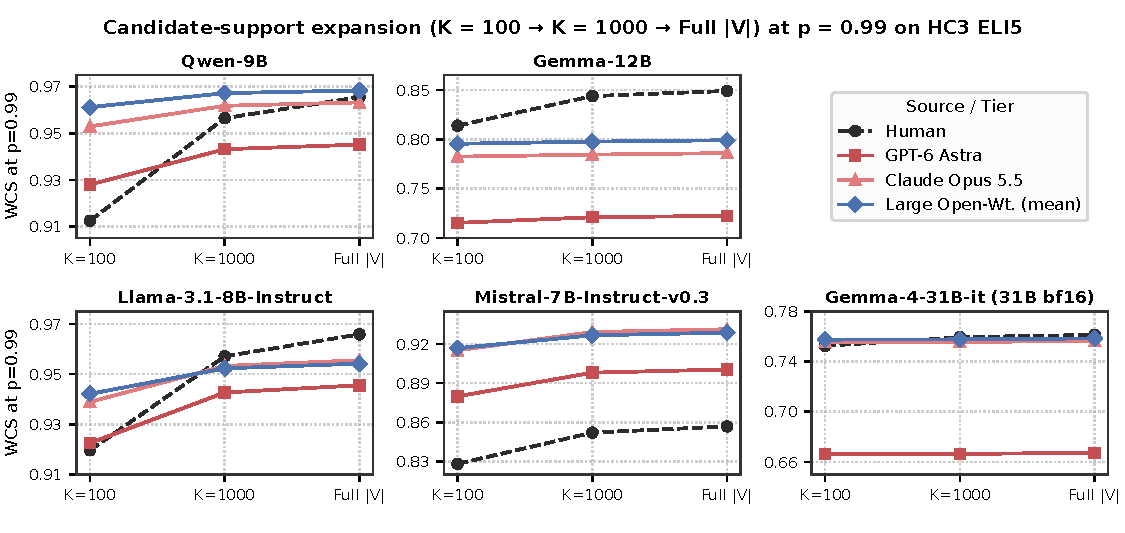
\includegraphics[width=0.96\textwidth]{figures_nov2/fig6_support_expansion.pdf}
\caption{Candidate-support expansion from $K=100$ to $K=1000$ to exact full vocabulary ($|V|$) at $p=0.99$ on HC3 ELI5 across Qwen-9B, Gemma-12B, Llama-3.1-8B, and Mistral-7B. Human writing exhibits the steepest upward trajectory from $K=100$ to $K=1000$ because human lexical choices frequently sit at token ranks $101$--$1000$ while remaining inside the $p=0.99$ full-vocabulary nucleus.}
\label{fig:support_expansion}
\end{figure*}

\begin{table*}[t]
\centering
\small
\resizebox{\textwidth}{!}{%
\begin{tabular}{lccccccc}
\toprule
Source / Tier & Tail Mass ($K=100$) & Tail Mass ($K=1000$) & Miss\% ($K=100$) & Miss\% ($K=1000$) & WCS ($K=100$) & WCS ($K=1000$) & WCS (\texttt{strict\_full} / \% Gap Closed) \\
\midrule
\multicolumn{8}{l}{\textit{Qwen3.5-9B Scorer ($|V| = 248{{,}}320$)}} \\
Human (HC3 ELI5, detok.) & 2.44\% & 0.416\% & 4.77\% & 0.72\% & 0.9124 & 0.9565 & 0.9655 (82.9\%) \\
GPT-6 Astra & 0.47\% & 0.054\% & 1.70\% & 0.10\% & 0.9279 & 0.9432 & 0.9451 (88.5\%) \\
Claude Opus 5.5 & 0.37\% & 0.048\% & 0.76\% & 0.03\% & 0.9529 & 0.9618 & 0.9633 (85.8\%) \\
Gemini 4 Argon & 0.26\% & 0.031\% & 0.83\% & 0.06\% & 0.9509 & 0.9575 & 0.9587 (84.6\%) \\
Frontier Proprietary (mean, 3 sources) & 0.37\% & 0.044\% & 1.10\% & 0.06\% & 0.9439 & 0.9541 & 0.9557 (86.9\%) \\
Large Open-Weight (mean, 7 sources) & 0.30\% & 0.036\% & 0.64\% & 0.05\% & 0.9612 & 0.9672 & 0.9684 (84.3\%) \\
Small Open-Weight (mean, 5 core sources) & 0.16\% & 0.018\% & 0.07\% & 0.00\% & 0.9903 & 0.9913 & 0.9916 (80.0\%) \\
\midrule
\multicolumn{8}{l}{\textit{Gemma-4-12B-it Scorer ($|V| = 262{{,}}144$)}} \\
Human (HC3 ELI5, detok.) & 0.90\% & 0.080\% & 6.75\% & 1.56\% & 0.8138 & 0.8437 & 0.8489 (85.0\%) \\
GPT-6 Astra & 0.05\% & 0.003\% & 3.66\% & 0.52\% & 0.7154 & 0.7210 & 0.7225 (79.3\%) \\
Claude Opus 5.5 & 0.03\% & 0.002\% & 1.52\% & 0.18\% & 0.7824 & 0.7845 & 0.7860 (57.3\%) \\
Gemini 4 Argon & 0.01\% & 0.001\% & 0.96\% & 0.09\% & 0.8128 & 0.8137 & 0.8145 (51.3\%) \\
Frontier Proprietary (mean, 3 sources) & 0.03\% & 0.002\% & 2.05\% & 0.26\% & 0.7702 & 0.7731 & 0.7743 (69.2\%) \\
Large Open-Weight (mean, 7 sources) & 0.02\% & 0.001\% & 1.49\% & 0.21\% & 0.7954 & 0.7976 & 0.7990 (61.3\%) \\
Small Open-Weight (mean, 5 core sources) & 0.01\% & 0.000\% & 0.19\% & 0.01\% & 0.9115 & 0.9120 & 0.9128 (42.2\%) \\
\midrule
\multicolumn{8}{l}{\textit{Llama-3.1-8B-Instruct Scorer ($|V| = 128{{,}}256$)}} \\
Human (HC3 ELI5, detok.) & 3.47\% & 0.669\% & 4.42\% & 0.78\% & 0.9196 & 0.9571 & 0.9659 (81.0\%) \\
GPT-6 Astra & 1.21\% & 0.168\% & 2.42\% & 0.22\% & 0.9225 & 0.9427 & 0.9455 (87.5\%) \\
Claude Opus 5.5 & 0.85\% & 0.126\% & 1.56\% & 0.08\% & 0.9389 & 0.9533 & 0.9555 (86.3\%) \\
Gemini 4 Argon & 0.61\% & 0.092\% & 1.35\% & 0.09\% & 0.9394 & 0.9519 & 0.9539 (86.0\%) \\
Frontier Proprietary (mean, 3 sources) & 0.89\% & 0.128\% & 1.78\% & 0.13\% & 0.9336 & 0.9493 & 0.9517 (86.8\%) \\
Large Open-Weight (mean, 7 sources) & 0.68\% & 0.101\% & 1.07\% & 0.08\% & 0.9421 & 0.9523 & 0.9542 (84.3\%) \\
Small Open-Weight (mean, 5 core sources) & 0.26\% & 0.033\% & 0.26\% & 0.01\% & 0.9629 & 0.9660 & 0.9666 (82.4\%) \\
\midrule
\multicolumn{8}{l}{\textit{Mistral-7B-Instruct-v0.3 Scorer ($|V| = 32{{,}}768$)}} \\
Human (HC3 ELI5, detok.) & 0.52\% & 0.065\% & 5.23\% & 0.98\% & 0.8281 & 0.8520 & 0.8568 (83.3\%) \\
GPT-6 Astra & 0.35\% & 0.040\% & 2.14\% & 0.19\% & 0.8799 & 0.8980 & 0.9005 (88.0\%) \\
Claude Opus 5.5 & 0.30\% & 0.036\% & 1.44\% & 0.12\% & 0.9152 & 0.9292 & 0.9313 (86.7\%) \\
Gemini 4 Argon & 0.26\% & 0.039\% & 1.70\% & 0.18\% & 0.9154 & 0.9261 & 0.9278 (86.1\%) \\
Frontier Proprietary (mean, 3 sources) & 0.30\% & 0.038\% & 1.76\% & 0.16\% & 0.9035 & 0.9178 & 0.9199 (87.1\%) \\
Large Open-Weight (mean, 7 sources) & 0.26\% & 0.033\% & 1.17\% & 0.13\% & 0.9168 & 0.9267 & 0.9287 (83.0\%) \\
Small Open-Weight (mean, 5 core sources) & 0.16\% & 0.020\% & 0.49\% & 0.04\% & 0.9472 & 0.9512 & 0.9523 (78.5\%) \\
\bottomrule
\end{tabular}%
}
\caption{Candidate-support validation comparing $K=100$, $K=1000$, and exact full-vocabulary nucleus scoring (\texttt{strict\_full}) at $p=0.99$ on HC3 ELI5 across four scorer families (Qwen3.5-9B, Gemma-4-12B-it, Llama-3.1-8B-Instruct, and Mistral-7B-Instruct-v0.3). ``\% Gap Closed'' reports $(\text{WCS}_{1000} - \text{WCS}_{100}) / (\text{WCS}_{\text{full}} - \text{WCS}_{100})$.}
\label{tab:top1000}
\end{table*}

Why does Human writing score lower than Frontier Proprietary text under realistic $K=100$ filtering ($0.8374$ vs.\ $0.8627$), yet slightly \emph{higher} under \texttt{strict\_full} ($0.8784$ vs.\ $0.8730$, Tables~\ref{tab:tiers} and~\ref{tab:eli5_strict_full})? Figure~\ref{fig:support_expansion} and Table~\ref{tab:top1000} resolve this mechanism directly. When scoring human text, a flat predictive distribution often spreads the $0.99$ probability nucleus across hundreds of plausible continuation tokens; a human word whose token ranks between $101$ and $1000$ has cumulative preceding mass $\le 0.99$ (so it survives \texttt{strict\_full}), but is deterministically clipped by the $K=100$ rank cap.

Expanding stored candidate support from $K=100$ to $K=1000$ reduces top-$K$ token misses on human writing from $4.77\%$ to $0.72\%$ on Qwen-9B (closing $82.9\%$ of the WCS gap to \texttt{strict\_full}: $0.9124 \to 0.9565$ vs.\ $0.9655$) and from $6.75\%$ to $1.56\%$ on Gemma-12B (closing $85.0\%$ of the gap: $0.8138 \to 0.8437$ vs.\ $0.8489$). Extending the $K=1000$ validation to Llama-3.1-8B-Instruct ($|V|=128{,}256$) and Mistral-7B-Instruct-v0.3 ($|V|=32{,}768$) confirms the same mechanism across all four model families: on human ELI5 responses, expanding support from $K=100$ to $K=1000$ reduces top-$K$ miss rates from $4.42\%$ to $0.78\%$ on Llama-3.1-8B (closing $81.0\%$ of the WCS gap to \texttt{strict\_full}: $0.9196 \to 0.9571$ vs.\ $0.9659$) and from $5.23\%$ to $0.98\%$ on Mistral-7B (closing $83.3\%$ of the WCS gap: $0.8281 \to 0.8520$ vs.\ $0.8568$). By contrast, Small Open-Weight sources experience $<0.2\%$ top-$100$ misses on Qwen and Gemma because their greedy tokens almost always reside in the top-$20$ head.

\subsection{Cross-Family Generalization and Same-Family Advantage}

\begin{figure}[t]
\centering
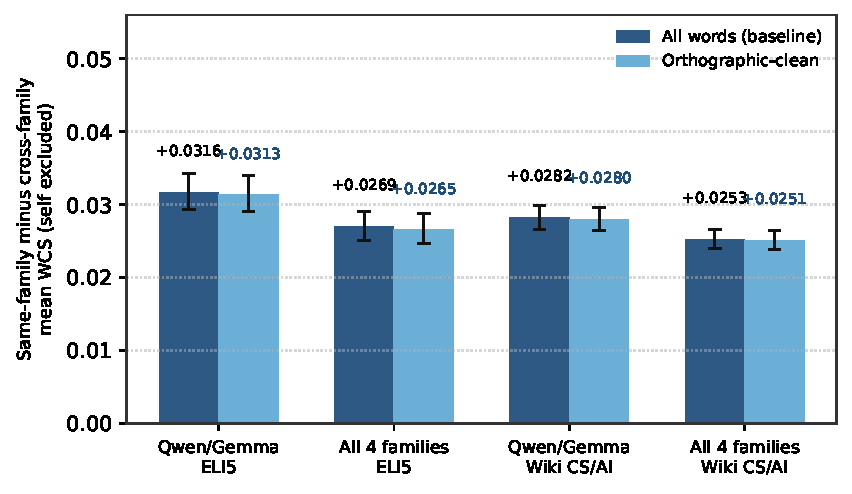
\includegraphics[width=\columnwidth]{figures_nov2/fig7_same_family.pdf}
\caption{Off-diagonal Same-Family Advantage (mean WCS on same-family open-weight pairs minus cross-family open-weight pairs, excluding self-scoring $s=g$) at $p=0.99$ with 95\% prompt-paired bootstrap confidence intervals, shown before (dark blue) and after (light blue) excluding family-specific orthographic confounds (curly apostrophes, standalone em-dashes, and \texttt{alright}).}
\label{fig:same_family}
\end{figure}

\begin{table*}[t]
\centering
\small
\resizebox{\textwidth}{!}{%
\begin{tabular}{lccccccccccc}
\toprule
Source Generator & Qwen-4B & Qwen-9B & Qwen-27B & Qwen-32B & Gemma-E4B & Gemma-12B & Llama-1B & Llama-8B & Mistral-7B & 7-bf16 Mean & 9-Scorer Mean \\
\midrule
\multicolumn{12}{l}{\textit{Human Reference}} \\
Human (HC3 ELI5, detok.) & 0.91 & 0.91 & 0.92 & 0.90 & 0.72 & 0.81 & 0.88 & 0.92 & 0.83 & 0.8545 & 0.8669 \\
\midrule
\multicolumn{12}{l}{\textit{Frontier Proprietary}} \\
GPT-6 Astra & 0.92 & 0.93 & 0.92 & 0.91 & 0.74 & 0.72 & 0.89 & 0.92 & 0.88 & 0.8560 & 0.8685 \\
Claude Opus 5.5 & 0.95 & 0.95 & 0.95 & 0.94 & 0.81 & 0.78 & 0.91 & 0.94 & 0.92 & 0.8934 & 0.9047 \\
Gemini 4 Argon & 0.95 & 0.95 & 0.94 & 0.94 & 0.84 & 0.81 & 0.92 & 0.94 & 0.92 & 0.9047 & 0.9125 \\
\midrule
\multicolumn{12}{l}{\textit{Large Open-Weight}} \\
DeepSeek-V4.1-Flash & 0.95 & 0.96 & 0.95 & 0.93 & 0.80 & 0.76 & 0.90 & 0.94 & 0.90 & 0.8850 & 0.8974 \\
GLM-5.3 & 0.95 & 0.96 & 0.95 & 0.94 & 0.81 & 0.79 & 0.90 & 0.94 & 0.92 & 0.8941 & 0.9060 \\
MiniMax-M3 & 0.95 & 0.96 & 0.95 & 0.94 & 0.82 & 0.79 & 0.91 & 0.94 & 0.91 & 0.8978 & 0.9076 \\
Kimi-K3 & 0.95 & 0.96 & 0.95 & 0.94 & 0.83 & 0.79 & 0.90 & 0.94 & 0.92 & 0.8980 & 0.9088 \\
MiMo-V2.6-Pro & 0.96 & 0.96 & 0.96 & 0.95 & 0.85 & 0.80 & 0.92 & 0.94 & 0.92 & 0.9085 & 0.9180 \\
DeepSeek-V4-Pro & 0.96 & 0.96 & 0.96 & 0.95 & 0.85 & 0.81 & 0.92 & 0.95 & 0.92 & 0.9100 & 0.9194 \\
Qwen3.8-2.4T-A95B & 0.97 & 0.97 & 0.96 & 0.96 & 0.87 & 0.84 & 0.93 & 0.95 & 0.93 & 0.9211 & 0.9299 \\
\midrule
\multicolumn{12}{l}{\textit{Small Open-Weight (4 Families)}} \\
Qwen-4B & \textbf{1.00} & 1.00 & 0.99 & 0.96 & 0.93 & 0.88 & 0.96 & 0.97 & 0.95 & 0.9562 & 0.9604 \\
Qwen-9B & 1.00 & \textbf{1.00} & 0.99 & 0.97 & 0.93 & 0.89 & 0.95 & 0.97 & 0.95 & 0.9554 & 0.9610 \\
Qwen-27B (int8) & 1.00 & 1.00 & \textbf{1.00} & 0.97 & 0.94 & 0.91 & 0.95 & 0.96 & 0.95 & 0.9577 & 0.9637 \\
Qwen2.5-32B (int8) & 0.98 & 0.98 & 0.97 & \textbf{1.00} & 0.91 & 0.86 & 0.96 & 0.97 & 0.96 & 0.9441 & 0.9530 \\
Gemma-E4B & 0.98 & 0.97 & 0.96 & 0.96 & \textbf{1.00} & 0.88 & 0.94 & 0.96 & 0.94 & 0.9538 & 0.9554 \\
Gemma-12B & 0.98 & 0.98 & 0.98 & 0.96 & 0.94 & \textbf{1.00} & 0.94 & 0.95 & 0.94 & 0.9626 & 0.9638 \\
Llama-3.2-1B & 0.98 & 0.97 & 0.97 & 0.95 & 0.85 & 0.90 & \textbf{1.00} & 0.99 & 0.94 & 0.9464 & 0.9497 \\
Llama-3.1-8B & 0.99 & 0.98 & 0.98 & 0.98 & 0.90 & 0.92 & 1.00 & \textbf{1.00} & 0.98 & 0.9664 & 0.9704 \\
Mistral-7B-v0.3 & 0.98 & 0.98 & 0.98 & 0.98 & 0.88 & 0.90 & 0.98 & 0.99 & \textbf{1.00} & 0.9571 & 0.9619 \\
\bottomrule
\end{tabular}%
}
\caption{Four-family expanded cross-model WCS matrix on HC3 ELI5 under realistic nucleus filtering ($p=0.99, K=100$) across $9$ scorers ($7$ \texttt{bf16} + $2$ \texttt{int8}) and $20$ sources.}
\label{tab:eli5_4family}
\end{table*}

Table~\ref{tab:eli5_4family} expands the HC3 ELI5 audit to $9$ scorers and $20$ sources across four model families (Qwen, Gemma, Llama, and Mistral). Across all $9$ scorers (and across the $7$ unquantized \texttt{bf16} scorers), the four-tier ordering holds without exception: Human ($0.8669$ 9-scorer; $0.8545$ 7-bf16) $<$ Frontier Proprietary ($0.8952$; $0.8847$) $<$ Large Open-Weight ($0.9124$; $0.9020$) $<$ Small Open-Weight ($0.9599$; $0.9555$), with Large minus Small Open-Weight $\Delta = -0.0476$ (95\% CI $[-0.0504,\,-0.0447]$) and Large minus Frontier Proprietary $\Delta = +0.0172$ (95\% CI $[+0.0152,\,+0.0192]$).

\paragraph{Same-Family Advantage and Orthographic Sensitivity Check.}
Excluding self-scoring diagonal cells ($s \neq g$), scorers exhibit a consistent \textbf{Same-Family Advantage} over cross-family open-weight sources (Figure~\ref{fig:same_family}):
\begin{itemize}
    \item Across Qwen and Gemma pairs on ELI5 ($n=18$ same-family vs.\ $36$ cross-family pairs, including \texttt{qwen3.8-2.4t-a95b} as a Qwen source), same-family pairs exceed cross-family pairs at $p=0.99$ by $\Delta = +0.0316$ (95\% CI $[+0.0294,\,+0.0343]$; rounded-cell $\Delta = +0.0328$), widening to $+0.0485$ ($[+0.0457,\,+0.0518]$) at $p=0.95$ and $+0.0552$ ($[+0.0519,\,+0.0589]$) at $p=0.90$.
    \item Across all four families on ELI5 ($n=20$ same-family vs.\ $61$ cross-family pairs), the Same-Family Advantage is $\Delta = +0.0269$ at $p=0.99$ (95\% CI $[+0.0251,\,+0.0291]$; rounded-cell $\Delta = +0.0286$), rising to $+0.0471$ ($[+0.0449,\,+0.0495]$) at $p=0.95$ and $+0.0580$ ($[+0.0553,\,+0.0607]$) at $p=0.90$.
    \item \textbf{Orthographic confound exclusion:} Because Appendix~\ref{app:zipf} identifies family-specific orthographic habits—such as Gemma 4's Unicode curly apostrophes (\texttt{U+2019} in \texttt{it's}, \texttt{let's}), Mistral-7B's conversational opener \texttt{Alright,}, and standalone em-dashes (\texttt{---})—we recomputed the Same-Family Advantage after excluding all words containing curly apostrophes, standalone punctuation/em-dashes, or \texttt{alright}. The Same-Family Advantage remains $+0.0313$ ($[+0.0290,\,+0.0340]$, $99.0\%$ preserved) for Qwen/Gemma and $+0.0265$ ($[+0.0246,\,+0.0287]$, $98.4\%$ preserved) across all four families at $p=0.99$, demonstrating that intra-family affinity reflects broad lexical alignment rather than punctuation artifacts.
\end{itemize}

\subsection{Cross-Domain Replication on Wikipedia CS/AI}

\begin{table*}[t]
\centering
\small
\resizebox{\textwidth}{!}{%
\begin{tabular}{lccccccccc}
\toprule
Source Generator & Qwen-4B & Qwen-9B & Gemma-E4B & Gemma-12B & Llama-1B & Llama-8B & Mistral-7B & 4-bf16 Mean & 7-bf16 Mean \\
\midrule
\multicolumn{10}{l}{\textit{Human Reference}} \\
Human (Wikipedia CS/AI) & 0.93 & 0.95 & 0.74 & 0.81 & 0.90 & 0.94 & 0.89 & 0.8569 & 0.8799 \\
\midrule
\multicolumn{10}{l}{\textit{Frontier Proprietary}} \\
GPT-6 Astra & 0.94 & 0.95 & 0.76 & 0.78 & 0.91 & 0.94 & 0.90 & 0.8589 & 0.8844 \\
Claude Opus 5.5 & 0.95 & 0.96 & 0.81 & 0.81 & 0.92 & 0.95 & 0.92 & 0.8828 & 0.9025 \\
Gemini 4 Argon & 0.96 & 0.95 & 0.86 & 0.86 & 0.93 & 0.95 & 0.93 & 0.9087 & 0.9199 \\
\midrule
\multicolumn{10}{l}{\textit{Large Open-Weight}} \\
DeepSeek-V4.1-Flash & 0.95 & 0.96 & 0.79 & 0.79 & 0.92 & 0.94 & 0.91 & 0.8716 & 0.8934 \\
GLM-5.3 & 0.96 & 0.96 & 0.85 & 0.83 & 0.93 & 0.95 & 0.93 & 0.9007 & 0.9165 \\
MiniMax-M3 & 0.97 & 0.97 & 0.87 & 0.85 & 0.93 & 0.96 & 0.95 & 0.9128 & 0.9269 \\
Kimi-K3 & 0.96 & 0.96 & 0.83 & 0.83 & 0.92 & 0.95 & 0.93 & 0.8953 & 0.9108 \\
MiMo-V2.6-Pro & 0.97 & 0.97 & 0.87 & 0.85 & 0.93 & 0.96 & 0.95 & 0.9157 & 0.9286 \\
DeepSeek-V4-Pro & 0.96 & 0.96 & 0.85 & 0.84 & 0.93 & 0.95 & 0.93 & 0.9022 & 0.9166 \\
Qwen3.8-2.4T-A95B & 0.98 & 0.98 & 0.90 & 0.88 & 0.94 & 0.96 & 0.95 & 0.9313 & 0.9412 \\
\midrule
\multicolumn{10}{l}{\textit{Small Open-Weight (4 Families)}} \\
Qwen-4B & \textbf{1.00} & 1.00 & 0.93 & 0.91 & 0.96 & 0.97 & 0.96 & 0.9572 & 0.9593 \\
Qwen-9B & 1.00 & \textbf{1.00} & 0.93 & 0.91 & 0.96 & 0.97 & 0.96 & 0.9595 & 0.9612 \\
Gemma-E4B & 0.98 & 0.97 & \textbf{1.00} & 0.90 & 0.95 & 0.96 & 0.95 & 0.9604 & 0.9572 \\
Gemma-12B & 0.98 & 0.97 & 0.94 & \textbf{1.00} & 0.95 & 0.96 & 0.94 & 0.9734 & 0.9630 \\
Llama-3.2-1B & 0.98 & 0.98 & 0.81 & 0.91 & \textbf{1.00} & 0.99 & 0.97 & 0.9229 & 0.9502 \\
Llama-3.1-8B & 0.99 & 0.99 & 0.83 & 0.92 & 1.00 & \textbf{1.00} & 0.99 & 0.9311 & 0.9581 \\
Mistral-7B-v0.3 & 0.99 & 0.99 & 0.85 & 0.91 & 0.98 & 0.99 & \textbf{1.00} & 0.9322 & 0.9562 \\
\bottomrule
\end{tabular}%
}
\caption{Cross-domain replication on HC3 Wikipedia CS/AI ($N=50$ prompts) under realistic nucleus filtering ($p=0.99, K=100$).}
\label{tab:wiki}
\end{table*}

Table~\ref{tab:wiki} and Table~\ref{tab:tiers} replicate our audit on technical encyclopedia prompts from HC3 Wikipedia CS/AI ($N=50$). Across the $4$ core \texttt{bf16} scorers and $15$ sources, the four-tier ordering replicates with slightly higher baseline reachability due to standardized technical terminology: Human ($0.8569$) $<$ Frontier Proprietary ($0.8835$; Human minus Frontier $\Delta = -0.0266$, 95\% CI $[-0.0325,\,-0.0205]$) $<$ Large Open-Weight ($0.9042$; Large minus Frontier $\Delta = +0.0207$, 95\% CI $[+0.0182,\,+0.0233]$) $<$ Small Open-Weight ($0.9626$; Large minus Small $\Delta = -0.0584$, 95\% CI $[-0.0616,\,-0.0552]$). Just as on ELI5, switching to exact full-vocabulary nucleus scoring (\texttt{strict\_full}, $p=0.99$) eliminates the gap between Human ($0.8868$) and Frontier Proprietary ($0.8897$; $\Delta = -0.0029$, 95\% CI $[-0.0084,\,+0.0024]$) while preserving the $-0.0549$ separation between Large and Small Open-Weight tiers. Extending Wikipedia CS/AI across all four scorer families (7 bf16 open-weight scorers and 18 sources, adding Llama-3.2-1B-Instruct, Llama-3.1-8B-Instruct, and Mistral-7B-Instruct-v0.3) preserves the identical four-tier ordering: at $p=0.99$, mean WCS rises from Human ($0.8799$) to Frontier Proprietary ($0.9023$) to Large Open-Weight ($0.9191$) to Small Open-Weight ($0.9579$), with Large Open-Weight minus Small Open-Weight $\Delta = -0.0387$ ($[-0.0417,\,-0.0360]$) and Large Open-Weight minus Frontier Proprietary $\Delta = +0.0169$ ($[+0.0148,\,+0.0189]$). Across all four families on Wikipedia CS/AI ($n=8$ same-family vs.\ $41$ cross-family pairs), the off-diagonal Same-Family Advantage is $\Delta = +0.0253$ ($[+0.0240,\,+0.0266]$; rounded-cell $\Delta = +0.0279$), and remains $+0.0251$ ($[+0.0238,\,+0.0264]$) after orthographic confound exclusion.

\subsection{Decoding Regime Ablation: Greedy vs.\ Sampled ($T>0$) Local Sources}

\begin{table*}[t]
\centering
\small
\resizebox{\textwidth}{!}{%
\begin{tabular}{lccccccc}
\toprule
Source Generator & Qwen-4B & Qwen-9B & Gemma-E4B & Gemma-12B & Sampled Mean & Greedy Mean & Sampled $-$ Greedy $\Delta$ \\
\midrule
Human (HC3 ELI5, detok.) & 0.91 & 0.91 & 0.72 & 0.81 & 0.8374 & 0.8374 & --- \\
Qwen-4B (sampled $T=1.0, p=0.95$) & \textbf{1.00} & 0.99 & 0.90 & 0.86 & 0.9396 & 0.9524 & $-0.0129$ \\
Qwen-9B (sampled $T=1.0, p=0.95$) & 1.00 & \textbf{1.00} & 0.91 & 0.87 & 0.9449 & 0.9538 & $-0.0089$ \\
Gemma-12B (sampled $T=1.0, p=0.95$) & 0.98 & 0.98 & 0.93 & \textbf{1.00} & 0.9739 & 0.9764 & $-0.0026$ \\
Gemma-E4B (sampled $T=1.0, p=0.95$) & 0.97 & 0.96 & \textbf{1.00} & 0.85 & 0.9470 & 0.9583 & $-0.0113$ \\
GPT-6 Astra & 0.92 & 0.93 & 0.74 & 0.72 & 0.8255 & 0.8255 & --- \\
Claude Opus 5.5 & 0.95 & 0.95 & 0.81 & 0.78 & 0.8728 & 0.8728 & --- \\
Gemini 4 Argon & 0.95 & 0.95 & 0.84 & 0.81 & 0.8897 & 0.8897 & --- \\
\bottomrule
\end{tabular}%
}
\caption{Stochastic-regeneration decoding ablation on HC3 ELI5 (realistic $p=0.99, K=100$, detokenized human reference). Local open-weight sources are regenerated using ancestral nucleus sampling ($T=1.0, p=0.95$) matched to the API sampling regime of Frontier Proprietary and Large Open-Weight models.}
\label{tab:sampled}
\end{table*}

A natural concern is that in our primary baseline, local Small Open-Weight sources are decoded greedily whereas API-hosted Frontier Proprietary and Large Open-Weight sources use stochastic nucleus sampling ($T=1.0, p=0.95$). To isolate generator tier from decoding stochasticity, Table~\ref{tab:sampled} regenerates all four \texttt{bf16} local sources on HC3 ELI5 under matched stochastic sampling ($T=1.0, p=0.95$). Sampling reduces Small Open-Weight reachability by only $0.0040$ to $0.0156$ per model (tier mean $0.9513$ vs.\ $0.9602$ greedy), leaving a $-0.0652$ gap below Large Open-Weight ($0.8862$, 95\% CI $[-0.0687,\,-0.0617]$) and a $-0.0887$ gap below Frontier Proprietary ($0.8627$). Thus, $>88\%$ of the reachability gap between Small Open-Weight and larger tiers persists when all generators share the exact same $T=1.0, p=0.95$ sampling regime.

\section{Discussion and High-VRAM Extension}

\paragraph{Why Does Reachability Track Generator Tier?}
Our experiments separate two distinct mechanisms governing cross-model lexical reachability:
\begin{enumerate}
    \item \textbf{Tail breadth vs.\ top-$K$ rank truncation (Human vs.\ Frontier):} Human writers and Frontier Proprietary models (especially GPT-6 Astra) select contextually appropriate synonyms, metaphors, and domain terms that disperse probability mass across $>100$ subword candidates. These choices survive an exact $p=0.99$ full-vocabulary nucleus (\texttt{strict\_full}), where Human and Frontier Proprietary reachability coincide ($0.8784$ vs.\ $0.8730$ on ELI5; $0.8868$ vs.\ $0.8897$ on Wikipedia), but are disproportionately clipped by top-$100$ rank caps.
    \item \textbf{Mode concentration in open-weight post-training (Small vs.\ Large Open-Weight):} Small Open-Weight models ($1.2\text{B}$--$32.5\text{B}$) concentrate their generations inside a high-probability lexical core that every other open-weight family also assigns to its top-$20$ candidates—even under stochastic $T=1.0, p=0.95$ sampling and under \texttt{strict\_full}. Large Open-Weight MoE models ($427\text{B}$--$2.78\text{T}$) occupy a consistent intermediate tier between Frontier Proprietary and Small Open-Weight models across both domains and all nine filter regimes.
\end{enumerate}

\paragraph{High-VRAM Turnkey Pipeline for \texttt{Gemma-4-31B-it}.}
While \texttt{Qwen3.5-27B} and \texttt{Qwen2.5-32B-Instruct} are evaluated in 8-bit quantization on our $47.5\text{ GiB}$ GPU slice, evaluating \texttt{google/gemma-4-31B-it} ($31.3\text{B}$ parameters, revision \texttt{842da379}) in unquantized \texttt{bf16} requires $\sim 57.7\text{ GiB}$ for model weights plus KV-cache headroom ($\ge 80\text{ GiB}$ GPU). In accordance with our reproducibility protocol—which prohibits silently substituting lower precision for a designated \texttt{bf16} scorer—we provide \texttt{scripts/run\_high\_vram\_server.sh} and dedicated configurations (\texttt{configs/high-vram-*.yaml}) to execute \texttt{Gemma-4-31B-it} generation, $K=100$ matrix scoring on ELI5 and Wikipedia CS/AI, and $K=1000$ validation on an 80GB/94GB server and automatically merge the resulting cells into all paper tables and figures.

\section{Conclusion}
We presented a comprehensive cross-model audit of lexical reachability using the Word Coverage Score across $20$ generators, $9$ open-weight scorers spanning four model families, two HC3 domains, and nine candidate-pool filter regimes. By pairing standard top-$K$ nucleus audits with $K=1000$ support expansion, exact full-vocabulary \texttt{strict\_full} scoring, stochastic-regeneration ablations, and a Zipf-adjusted lexical loss taxonomy, we showed that top-$K$ rank truncation explains the apparent reachability deficit of human writing relative to frontier proprietary models, while a robust structural gap separates human and frontier prose from the highly concentrated vocabulary of small open-weight models.

\section*{Limitations}
Our teacher-forced WCS audit requires full logit and subword offset access, restricting the scorer role to open-weight checkpoints; proprietary frontier models can be audited as sources but not as scorers unless providers expose full-vocabulary log-probabilities. Second, our largest local checkpoints on the primary $47.5\text{ GiB}$ server (\texttt{Qwen3.5-27B-int8} and \texttt{Qwen2.5-32B-int8}) use 8-bit quantization, while unquantized \texttt{bf16} evaluation at the $\sim 30\text{B}$ scale (\texttt{Gemma-4-31B-it}) requires an 80GB/94GB GPU via our turnkey script. Finally, our benchmarks focus on English explanatory and technical prose ($150$--$400$ words); extending WCS matrices to morphologically rich languages and creative writing is an important direction for future work.

\section*{Ethical Considerations}
All human reference texts are drawn from the publicly released, anonymized HC3 benchmark \citep{guo2023hc3}. API generations were collected via standard commercial endpoints without logging credentials or personal data. Because WCS characterizes aggregate distributional overlap rather than providing a calibrated document-level classifier, it should not be used for high-stakes individual authorship attribution or academic misconduct adjudication.

\bibliography{references}

\clearpage
\appendix

\section{Additional Filter-Regime Matrices}
\label{app:matrices}

Tables~\ref{tab:eli5_shipped} and~\ref{tab:eli5_unscaled} report the full per-source and per-scorer HC3 ELI5 matrices under each scorer's shipped generation defaults and under unscaled ($T=1.0$) shipped top-$k$/top-$p$ filters.

\begin{table*}[h!]
\centering
\small
\resizebox{\textwidth}{!}{%
\begin{tabular}{lccccccc}
\toprule
Source Generator & Qwen-4B & Qwen-9B & Gemma-E4B & Gemma-12B & Qwen-27B (int8) & 4-bf16 Scorer Mean & Human $-$ Source $\Delta$ (95\% CI) \\
\midrule
\multicolumn{7}{l}{\textit{Human Reference}} \\
Human (HC3 ELI5, detok.) & 0.66 & 0.67 & 0.60 & 0.70 & 0.68 & 0.6591 & --- \\
\midrule
\multicolumn{7}{l}{\textit{Frontier Proprietary (API, $T=1.0, p=0.95$)}} \\
GPT-6 Astra & 0.66 & 0.69 & 0.62 & 0.60 & 0.70 & 0.6440 & $+0.0151$ ($[-0.0011,\,+0.0309]$) \\
Claude Opus 5.5 & 0.72 & 0.75 & 0.71 & 0.68 & 0.77 & 0.7181 & $-0.0590$ ($[-0.0731,\,-0.0453]$) \\
Gemini 4 Argon & 0.74 & 0.75 & 0.75 & 0.73 & 0.77 & 0.7414 & $-0.0823$ ($[-0.0973,\,-0.0679]$) \\
\midrule
\multicolumn{7}{l}{\textit{Large Open-Weight (API, $T=1.0, p=0.95$)}} \\
DeepSeek-V4.1-Flash & 0.72 & 0.75 & 0.69 & 0.65 & 0.76 & 0.7020 & $-0.0429$ ($[-0.0591,\,-0.0271]$) \\
GLM-5.3 & 0.73 & 0.75 & 0.71 & 0.68 & 0.77 & 0.7189 & $-0.0598$ ($[-0.0741,\,-0.0458]$) \\
MiniMax-M3 & 0.74 & 0.76 & 0.72 & 0.68 & 0.77 & 0.7259 & $-0.0668$ ($[-0.0818,\,-0.0518]$) \\
Kimi-K3 & 0.73 & 0.76 & 0.73 & 0.70 & 0.79 & 0.7305 & $-0.0715$ ($[-0.0875,\,-0.0546]$) \\
MiMo-V2.6-Pro & 0.75 & 0.77 & 0.75 & 0.71 & 0.78 & 0.7458 & $-0.0867$ ($[-0.1010,\,-0.0722]$) \\
DeepSeek-V4-Pro & 0.76 & 0.79 & 0.75 & 0.71 & 0.80 & 0.7515 & $-0.0924$ ($[-0.1090,\,-0.0761]$) \\
Qwen3.8-2.4T-A95B & 0.78 & 0.81 & 0.77 & 0.74 & 0.82 & 0.7770 & $-0.1180$ ($[-0.1327,\,-0.1039]$) \\
\midrule
\multicolumn{7}{l}{\textit{Small Open-Weight (Local Greedy)}} \\
Qwen-4B & \textbf{1.00} & 0.93 & 0.85 & 0.80 & 0.87 & 0.8923 & $-0.2332$ ($[-0.2479,\,-0.2191]$) \\
Qwen-9B & 0.93 & \textbf{1.00} & 0.85 & 0.80 & 0.90 & 0.8969 & $-0.2378$ ($[-0.2528,\,-0.2231]$) \\
Qwen-27B (int8) & 0.91 & 0.93 & 0.86 & 0.83 & \textbf{1.00} & 0.8827 & $-0.2236$ ($[-0.2385,\,-0.2091]$) \\
Gemma-12B & 0.84 & 0.84 & 0.86 & \textbf{1.00} & 0.85 & 0.8861 & $-0.2270$ ($[-0.2417,\,-0.2124]$) \\
Gemma-E4B & 0.83 & 0.81 & \textbf{1.00} & 0.79 & 0.80 & 0.8578 & $-0.1987$ ($[-0.2137,\,-0.1842]$) \\
\bottomrule
\end{tabular}%
}
\caption{HC3 ELI5 cross-model WCS matrix under each scorer's shipped generation defaults (Qwen 3.5: $T=0.6, k=20, p=0.95$; Gemma 4: $T=1.0, k=64, p=0.95$).}
\label{tab:eli5_shipped}
\end{table*}

\begin{table*}[h!]
\centering
\small
\resizebox{\textwidth}{!}{%
\begin{tabular}{lccccccc}
\toprule
Source Generator & Qwen-4B & Qwen-9B & Gemma-E4B & Gemma-12B & Qwen-27B (int8) & 4-bf16 Scorer Mean & Human $-$ Source $\Delta$ (95\% CI) \\
\midrule
\multicolumn{7}{l}{\textit{Human Reference}} \\
Human (HC3 ELI5, detok.) & 0.77 & 0.79 & 0.60 & 0.70 & 0.80 & 0.7157 & --- \\
\midrule
\multicolumn{7}{l}{\textit{Frontier Proprietary (API, $T=1.0, p=0.95$)}} \\
GPT-6 Astra & 0.79 & 0.81 & 0.62 & 0.60 & 0.82 & 0.7084 & $+0.0073$ ($[-0.0070,\,+0.0218]$) \\
Claude Opus 5.5 & 0.84 & 0.87 & 0.71 & 0.68 & 0.87 & 0.7758 & $-0.0601$ ($[-0.0731,\,-0.0476]$) \\
Gemini 4 Argon & 0.86 & 0.86 & 0.75 & 0.73 & 0.87 & 0.7983 & $-0.0826$ ($[-0.0966,\,-0.0689]$) \\
\midrule
\multicolumn{7}{l}{\textit{Large Open-Weight (API, $T=1.0, p=0.95$)}} \\
DeepSeek-V4.1-Flash & 0.85 & 0.87 & 0.69 & 0.65 & 0.87 & 0.7618 & $-0.0461$ ($[-0.0607,\,-0.0317]$) \\
GLM-5.3 & 0.85 & 0.87 & 0.71 & 0.68 & 0.88 & 0.7787 & $-0.0630$ ($[-0.0764,\,-0.0496]$) \\
MiniMax-M3 & 0.85 & 0.87 & 0.72 & 0.68 & 0.87 & 0.7834 & $-0.0677$ ($[-0.0811,\,-0.0541]$) \\
Kimi-K3 & 0.86 & 0.88 & 0.73 & 0.70 & 0.88 & 0.7897 & $-0.0740$ ($[-0.0884,\,-0.0587]$) \\
MiMo-V2.6-Pro & 0.87 & 0.89 & 0.75 & 0.71 & 0.89 & 0.8042 & $-0.0885$ ($[-0.1016,\,-0.0753]$) \\
DeepSeek-V4-Pro & 0.88 & 0.89 & 0.75 & 0.71 & 0.90 & 0.8070 & $-0.0913$ ($[-0.1065,\,-0.0762]$) \\
Qwen3.8-2.4T-A95B & 0.89 & 0.91 & 0.77 & 0.74 & 0.91 & 0.8292 & $-0.1135$ ($[-0.1269,\,-0.1003]$) \\
\midrule
\multicolumn{7}{l}{\textit{Small Open-Weight (Local Greedy)}} \\
Qwen-4B & \textbf{1.00} & 0.98 & 0.85 & 0.80 & 0.95 & 0.9061 & $-0.1904$ ($[-0.2038,\,-0.1774]$) \\
Qwen-9B & 0.98 & \textbf{1.00} & 0.85 & 0.80 & 0.97 & 0.9092 & $-0.1935$ ($[-0.2071,\,-0.1797]$) \\
Qwen-27B (int8) & 0.97 & 0.98 & 0.86 & 0.83 & \textbf{1.00} & 0.9119 & $-0.1962$ ($[-0.2096,\,-0.1829]$) \\
Gemma-12B & 0.93 & 0.93 & 0.86 & \textbf{1.00} & 0.93 & 0.9311 & $-0.2154$ ($[-0.2290,\,-0.2021]$) \\
Gemma-E4B & 0.92 & 0.91 & \textbf{1.00} & 0.79 & 0.90 & 0.9065 & $-0.1908$ ($[-0.2043,\,-0.1774]$) \\
\bottomrule
\end{tabular}%
}
\caption{HC3 ELI5 cross-model WCS matrix under unscaled ($T=1.0$) shipped top-$k$ and top-$p$ filters (Qwen 3.5: $T=1.0, k=20, p=0.95$; Gemma 4: $T=1.0, k=64, p=0.95$).}
\label{tab:eli5_unscaled}
\end{table*}

\section{Zipf-Adjusted Lexical Category and Loss-Rate Taxonomy}
\label{app:zipf}

To understand \emph{which} words fail the nucleus filter across generator tiers—and why raw counts of lost words can be misleading without frequency normalization—we conducted a word-level lexical audit across the expanded 4-family HC3 ELI5 evaluation suite ($9$ scorers evaluating $20$ sources at realistic $p=0.99$, excluding self-scoring diagonal pairs $s = g$, totaling $2{,}586{,}369$ off-diagonal word evaluations and $187{,}895$ lost word instances).

\paragraph{Methodology \& Word-Class Partition.}
For every off-diagonal scorer--source pair $(g, s)$ with $g \neq s$ and every prompt $q \in \{1, \dots, 50\}$, we align the whitespace word groups $W(y_{q,s})$ with the token-level survival mask under realistic $p=0.99$ ($K=100$). Each word instance $w$ is normalized by lowercasing and stripping leading/trailing ASCII punctuation (while preserving internal apostrophes and hyphens, and distinguishing ASCII straight apostrophes \texttt{'} from Unicode right single quotation marks \texttt{U+2019}) and assigned to one of three mutually exclusive macro-categories:
\begin{enumerate}
    \item \textbf{Function / Stopwords:} Standard closed-class English determiners, prepositions, conjunctions, auxiliary verbs, and pronouns ($85$ canonical forms).
    \item \textbf{Standalone Punctuation / Symbols:} Tokens consisting solely of non-alphanumeric characters bounded by whitespace (e.g., spaced em-dashes \texttt{---}, bullets, or markdown symbols \texttt{\#}, \texttt{>}).
    \item \textbf{Content / Lexical Words:} All remaining open-class nouns, lexical verbs, adjectives, adverbs, numbers, and hyphenated/contracted lexical forms.
\end{enumerate}
For each generator tier and each normalized word type $v$, we record total off-diagonal evaluations $N(v)$, total lost instances $L(v)$, and the \textbf{Zipf-adjusted per-occurrence loss rate} $r(v) = L(v)/N(v)$.

\begin{table*}[t]
\centering
\small
\resizebox{\textwidth}{!}{%
\begin{tabular}{llrrrr}
\toprule
Generator Tier & Word Macro-Category & Lost Words & Total Evaluated & Category Loss Rate & Share of Tier's Lost Words \\
\midrule
Human (HC3, 1 source) & Content / Lexical Words & 8,992 & 50,355 & 17.86\% & 77.4\% \\
 & Function / Stopwords & 2,461 & 39,384 & 6.25\% & 21.2\% \\
 & Standalone Punct. / Symbols & 167 & 630 & 26.51\% & 1.4\% \\
 & \textbf{Tier Total} & \textbf{11,620} & \textbf{90,369} & \textbf{12.86\%} & \textbf{100.0\%} \\
\midrule
Frontier Proprietary (3 sources) & Content / Lexical Words & 34,897 & 268,587 & 12.99\% & 77.4\% \\
 & Function / Stopwords & 9,959 & 169,281 & 5.88\% & 22.1\% \\
 & Standalone Punct. / Symbols & 210 & 3,078 & 6.82\% & 0.5\% \\
 & \textbf{Tier Total} & \textbf{45,066} & \textbf{440,946} & \textbf{10.22\%} & \textbf{100.0\%} \\
\midrule
Large Open-Weight (7 sources) & Content / Lexical Words & 61,714 & 579,573 & 10.65\% & 73.5\% \\
 & Function / Stopwords & 18,273 & 370,269 & 4.94\% & 21.8\% \\
 & Standalone Punct. / Symbols & 3,941 & 14,427 & 27.32\% & 4.7\% \\
 & \textbf{Tier Total} & \textbf{83,928} & \textbf{964,269} & \textbf{8.70\%} & \textbf{100.0\%} \\
\midrule
Small Open-Weight (9 sources, $s \neq g$) & Content / Lexical Words & 34,062 & 604,144 & 5.64\% & 71.7\% \\
 & Function / Stopwords & 13,242 & 487,664 & 2.72\% & 27.9\% \\
 & Standalone Punct. / Symbols & 198 & 2,136 & 9.27\% & 0.4\% \\
 & \textbf{Tier Total} & \textbf{47,502} & \textbf{1,093,944} & \textbf{4.34\%} & \textbf{100.0\%} \\
\bottomrule
\end{tabular}%
}
\caption{Macro-category breakdown of word losses at realistic $p=0.99$ across the 4-family HC3 ELI5 suite ($9$ scorers, $20$ sources, off-diagonal pairs $s \neq g$, $2{,}586{,}369$ word evaluations).}
\label{tab:zipf_macro}
\end{table*}

\begin{table*}[t]
\centering
\small
\resizebox{\textwidth}{!}{%
\begin{tabular}{lll}
\toprule
Generator Tier & Top Lost Words by Raw Count (Lost / Total, Loss Rate) & Top Lost Words by Loss Rate ($\ge 45$ Evals: Rate, Lost / Total) \\
\midrule
Human (HC3) &
\begin{tabular}[t]{@{}l@{}}
\texttt{the} ($139/4{,}725$, $2.9\%$), \texttt{a} ($109/2{,}520$, $4.3\%$), \texttt{and} ($106/2{,}025$, $5.2\%$),\\
\texttt{in} ($101/1{,}458$, $6.9\%$), \texttt{that} ($74/1{,}431$, $5.2\%$), \texttt{of} ($72/2{,}466$, $2.9\%$),\\
\texttt{i} ($72/333$, $21.6\%$), \texttt{this} ($68/648$, $10.5\%$), \texttt{from} ($63/504$, $12.5\%$)
\end{tabular} &
\begin{tabular}[t]{@{}l@{}}
\texttt{tl;dr} ($100.0\%$, $45/45$), \texttt{edit} ($77.8\%$, $42/54$), \texttt{depending} ($57.8\%$, $26/45$),\\
\texttt{whether} ($48.9\%$, $22/45$), \texttt{set} ($48.9\%$, $22/45$), \texttt{volume} ($48.9\%$, $22/45$),\\
\texttt{due} ($48.9\%$, $22/45$), \texttt{everybody} ($48.9\%$, $22/45$), \texttt{generally} ($46.7\%$, $21/45$)
\end{tabular} \\
\midrule
Frontier Prop. &
\begin{tabular}[t]{@{}l@{}}
\texttt{the} ($810/20{,}340$, $4.0\%$), \texttt{a} ($720/15{,}174$, $4.7\%$), \texttt{and} ($655/10{,}890$, $6.0\%$),\\
\texttt{that} ($411/4{,}833$, $8.5\%$), \texttt{your} ($376/4{,}734$, $7.9\%$), \texttt{it} ($306/7{,}002$, $4.4\%$),\\
\texttt{in} ($292/4{,}194$, $7.0\%$), \texttt{you} ($291/6{,}462$, $4.5\%$), \texttt{is} ($282/6{,}588$, $4.3\%$)
\end{tabular} &
\begin{tabular}[t]{@{}l@{}}
\texttt{acts} ($68.9\%$, $31/45$), \texttt{ordinary} ($68.7\%$, $68/99$), \texttt{surprise} ($57.4\%$, $31/54$),\\
\texttt{roughly} ($56.5\%$, $61/108$), \texttt{here's} ($54.0\%$, $68/126$), \texttt{recognize} ($53.3\%$, $24/45$),\\
\texttt{neither} ($51.9\%$, $28/54$), \texttt{electronic} ($51.1\%$, $23/45$), \texttt{plenty} ($51.1\%$, $23/45$)
\end{tabular} \\
\midrule
Large Open-Wt. &
\begin{tabular}[t]{@{}l@{}}
\texttt{---} ($3{,}190/7{,}092$, $45.0\%$), \texttt{the} ($1{,}804/43{,}128$, $4.2\%$), \texttt{a} ($1{,}276/31{,}005$, $4.1\%$),\\
\texttt{and} ($1{,}121/24{,}048$, $4.7\%$), \texttt{your} ($711/9{,}936$, $7.2\%$), \texttt{so} ($710/8{,}154$, $8.7\%$),\\
\texttt{that} ($704/10{,}872$, $6.5\%$), \texttt{here's} ($668/1{,}521$, $43.9\%$), \texttt{it} ($572/16{,}101$, $3.6\%$)
\end{tabular} &
\begin{tabular}[t]{@{}l@{}}
\texttt{\#} ($100.0\%$, $99/99$), \texttt{eli5} ($75.6\%$, $34/45$), \texttt{haitian} ($62.2\%$, $28/45$),\\
\texttt{honestly} ($59.7\%$, $43/72$), \texttt{deliberately} ($55.6\%$, $45/81$), \texttt{whose} ($54.2\%$, $39/72$),\\
\texttt{hanging} ($53.3\%$, $24/45$), \texttt{borrowed} ($51.9\%$, $28/54$), \texttt{great} ($50.9\%$, $357/702$)
\end{tabular} \\
\midrule
Small Open-Wt. &
\begin{tabular}[t]{@{}l@{}}
\texttt{the} ($997/56{,}080$, $1.8\%$), \texttt{and} ($710/25{,}384$, $2.8\%$), \texttt{is} ($640/21{,}216$, $3.0\%$),\\
\texttt{a} ($591/40{,}272$, $1.5\%$), \texttt{you} ($484/22{,}416$, $2.2\%$), \texttt{it} ($480/20{,}624$, $2.3\%$),\\
\texttt{to} ($444/30{,}904$, $1.4\%$), \texttt{so} ($442/6{,}528$, $6.8\%$), \texttt{imagine} ($375/3{,}680$, $10.2\%$)
\end{tabular} &
\begin{tabular}[t]{@{}l@{}}
\texttt{alright} ($88.1\%$, $155/176$), \texttt{let's} (curly, $56.3\%$, $27/48$), \texttt{removes} ($39.6\%$, $19/48$),\\
\texttt{poland} ($35.4\%$, $17/48$), \texttt{--} ($32.3\%$, $31/96$), \texttt{it's} (curly, $31.3\%$, $223/712$),\\
\texttt{asked} ($29.2\%$, $35/120$), \texttt{immediately} ($28.6\%$, $32/112$), \texttt{grown-ups} ($26.6\%$, $34/128$)
\end{tabular} \\
\bottomrule
\end{tabular}%
}
\caption{Comparison of top lost words ranked by raw failure count (left) versus Zipf-adjusted per-occurrence failure rate among words with $\ge 45$ evaluations (right) at realistic $p=0.99$ across the 9-scorer, 20-source 4-family ELI5 pool.}
\label{tab:zipf_words}
\end{table*}

\paragraph{Finding 1: Macro-Category Breakdown.}
Table~\ref{tab:zipf_macro} demonstrates that across all four generator tiers, \textbf{content/lexical words account for $71.7\%$--$77.4\%$ of all lost words} and suffer a per-occurrence loss rate $2.1\times$ to $2.9\times$ higher than function/stopwords:
\begin{itemize}
    \item In \textbf{Human} writing, $17.86\%$ of all content word tokens fail the $p=0.99$ filter ($8{,}992 / 50{,}355$), compared to only $6.25\%$ of function words ($2{,}461 / 39{,}384$).
    \item Across \textbf{Frontier Proprietary} ($12.99\%$ content vs.\ $5.88\%$ function), \textbf{Large Open-Weight} ($10.66\%$ content vs.\ $4.94\%$ function), and \textbf{Small Open-Weight} ($5.64\%$ content vs.\ $2.72\%$ function), the hierarchy of lexical reachability is driven primarily by a progressive $3.2\times$ contraction in content-word loss rates ($17.86\% \to 12.99\% \to 10.66\% \to 5.64\%$).
\end{itemize}

\paragraph{Finding 2: Raw-Count Leaders vs.\ Zipf-Adjusted Rate Leaders.}
Table~\ref{tab:zipf_words} contrasts the top lost words ranked by raw count against those ranked by per-occurrence loss rate ($\ge 45$ evaluations). Because function words like \texttt{the}, \texttt{a}, and \texttt{and} occur $20{,}000$--$56{,}000$ times per tier, even a $1.5\%$--$6.0\%$ failure rate produces hundreds to thousands of raw losses. Normalizing by occurrence frequency reveals the true high-risk lexical items: Reddit register markers (\texttt{tl;dr} $100\%$, \texttt{edit} $77.8\%$) and hedging words (\texttt{depending} $57.8\%$, \texttt{whether} $48.9\%$, \texttt{generally} $46.7\%$) in Human answers; nuanced verbs and qualifiers (\texttt{acts} $68.9\%$, \texttt{ordinary} $68.7\%$, \texttt{roughly} $56.5\%$) in Frontier Proprietary answers; markdown headers (\texttt{\#} $100\%$), conversational preambles (\texttt{eli5} $75.6\%$, \texttt{honestly} $59.7\%$, \texttt{great} $50.9\%$), and spaced em-dashes (\texttt{---} $45.0\%$) in Large Open-Weight answers; and family-specific openers/orthography (\texttt{alright} $88.1\%$, curly-apostrophe \texttt{let's} $56.3\%$ and \texttt{it's} $31.3\%$) in Small Open-Weight answers.

\paragraph{Finding 3: Why Function Words Still Fail Occasionally.}
Inspecting the $6{,}446$ total lost occurrences of \texttt{the} and \texttt{a} across the 9-scorer matrix reveals three concrete mechanisms: (i) \textbf{contextual phrase/idiom lock-in} ($39.0\%$, $2{,}513/6{,}446$), where the scorer assigns $\ge 0.95$ probability to a single fixed continuation token (e.g., an idiom or multi-word expression), pushing any alternative determiner past the $0.99$ boundary; (ii) \textbf{sentence-initial discourse framing} ($15.8\%$, $1{,}016/6{,}446$), where capitalized \texttt{The} or \texttt{A} competes against preferred bullet/discourse starters; and (iii) \textbf{mid-sentence determiner competition} ($45.3\%$, $2{,}917/6{,}446$), where a scorer strongly prefers a bare plural or possessive pronoun over an article.

\end{document}
